\documentclass[]{book}
\usepackage{lmodern}
\usepackage{amssymb,amsmath}
\usepackage{ifxetex,ifluatex}
\usepackage{fixltx2e} % provides \textsubscript
\ifnum 0\ifxetex 1\fi\ifluatex 1\fi=0 % if pdftex
  \usepackage[T1]{fontenc}
  \usepackage[utf8]{inputenc}
\else % if luatex or xelatex
  \ifxetex
    \usepackage{mathspec}
  \else
    \usepackage{fontspec}
  \fi
  \defaultfontfeatures{Ligatures=TeX,Scale=MatchLowercase}
\fi
% use upquote if available, for straight quotes in verbatim environments
\IfFileExists{upquote.sty}{\usepackage{upquote}}{}
% use microtype if available
\IfFileExists{microtype.sty}{%
\usepackage{microtype}
\UseMicrotypeSet[protrusion]{basicmath} % disable protrusion for tt fonts
}{}
\usepackage[margin=1in]{geometry}
\usepackage{hyperref}
\hypersetup{unicode=true,
            pdftitle={Book of Prob},
            pdfborder={0 0 0},
            breaklinks=true}
\urlstyle{same}  % don't use monospace font for urls
\usepackage{natbib}
\bibliographystyle{apalike}
\usepackage{longtable,booktabs}
\usepackage{graphicx,grffile}
\makeatletter
\def\maxwidth{\ifdim\Gin@nat@width>\linewidth\linewidth\else\Gin@nat@width\fi}
\def\maxheight{\ifdim\Gin@nat@height>\textheight\textheight\else\Gin@nat@height\fi}
\makeatother
% Scale images if necessary, so that they will not overflow the page
% margins by default, and it is still possible to overwrite the defaults
% using explicit options in \includegraphics[width, height, ...]{}
\setkeys{Gin}{width=\maxwidth,height=\maxheight,keepaspectratio}
\IfFileExists{parskip.sty}{%
\usepackage{parskip}
}{% else
\setlength{\parindent}{0pt}
\setlength{\parskip}{6pt plus 2pt minus 1pt}
}
\setlength{\emergencystretch}{3em}  % prevent overfull lines
\providecommand{\tightlist}{%
  \setlength{\itemsep}{0pt}\setlength{\parskip}{0pt}}
\setcounter{secnumdepth}{5}
% Redefines (sub)paragraphs to behave more like sections
\ifx\paragraph\undefined\else
\let\oldparagraph\paragraph
\renewcommand{\paragraph}[1]{\oldparagraph{#1}\mbox{}}
\fi
\ifx\subparagraph\undefined\else
\let\oldsubparagraph\subparagraph
\renewcommand{\subparagraph}[1]{\oldsubparagraph{#1}\mbox{}}
\fi

%%% Use protect on footnotes to avoid problems with footnotes in titles
\let\rmarkdownfootnote\footnote%
\def\footnote{\protect\rmarkdownfootnote}

%%% Change title format to be more compact
\usepackage{titling}

% Create subtitle command for use in maketitle
\newcommand{\subtitle}[1]{
  \posttitle{
    \begin{center}\large#1\end{center}
    }
}

\setlength{\droptitle}{-2em}
  \title{Book of Prob}
  \pretitle{\vspace{\droptitle}\centering\huge}
  \posttitle{\par}
  \author{}
  \preauthor{}\postauthor{}
  \date{}
  \predate{}\postdate{}

\usepackage{booktabs}
\usepackage{amsthm}
\makeatletter
\def\thm@space@setup{%
  \thm@preskip=8pt plus 2pt minus 4pt
  \thm@postskip=\thm@preskip
}
\makeatother

\usepackage{amsthm}
\newtheorem{theorem}{Theorem}[chapter]
\newtheorem{lemma}{Lemma}[chapter]
\theoremstyle{definition}
\newtheorem{definition}{Definition}[chapter]
\newtheorem{corollary}{Corollary}[chapter]
\newtheorem{proposition}{Proposition}[chapter]
\theoremstyle{definition}
\newtheorem{example}{Example}[chapter]
\theoremstyle{definition}
\newtheorem{exercise}{Exercise}[chapter]
\theoremstyle{remark}
\newtheorem*{remark}{Remark}
\newtheorem*{solution}{Solution}
\begin{document}
\maketitle

{
\setcounter{tocdepth}{1}
\tableofcontents
}
\hypertarget{introduction}{%
\chapter*{Introduction}\label{introduction}}
\addcontentsline{toc}{chapter}{Introduction}

This book is the combined lecture notes of my course IE-231 Introduction
to Probability at \href{https://www.bilgi.edu.tr}{Istanbul Bilgi
University}, Turkey. You can find the original lecture notes and
archives \href{https://berkorbay.github.io/bilgi-ie231/}{here}. As the
name suggests, these notes consist of an abbreviated version of the
course as the objective is to give the essence of very significant parts
of Probability. The course mainly follows \citep{myers2012}.

This book is periodically updated. Latest update is on 2018-05-07.

\hypertarget{about-the-author}{%
\section*{About the Author}\label{about-the-author}}
\addcontentsline{toc}{section}{About the Author}

The author of this book is \href{http://berkorbay.me}{Berk Orbay}. I am
the co-founder of \href{http://algopoly.com}{Algopoly}, a data science
firm specialized on large scale forecasting problems, and a part-time
academic (yes, still writing papers). My PhD was about pricing financial
options with multiple models. I taught or am currently teaching
Introduction to Probability, Computational Finance, Business Analytics
and Essentials of Data Analysis courses.

\hypertarget{acknowledgements}{%
\subsection*{Acknowledgements}\label{acknowledgements}}
\addcontentsline{toc}{subsection}{Acknowledgements}

Special thanks section.

\hypertarget{intro}{%
\chapter{Initial Concepts of Probability}\label{intro}}

\begin{itemize}
\item
  \textbf{Probability} is the quantification of event uncertainty. For
  instance, probability of getting (H)eads in a coin toss is \(1/2\).
  Deterministic models will give the same results given the same inputs
  (e.g.~2 times 2 is 4), but probabilistic models might yield different
  outcomes.
\item
  An \textbf{experiment} is a process that generates data. For instance,
  tossing a coin is an experiment. \textbf{Outcome} is the realization
  of an experiment. Possible outcomes for a coin toss is Heads and
  Tails.
\item
  \textbf{Sample space} (\(\mathbb{S}\)) is the collection of all the
  possible outcomes of an experiment. Sample space of the coin toss is
  \(\mathbb{S} = \{H,T\}\). Sample space of two coin tosses experiment
  is \(\mathbb{S} = \{HH,HT,TH,TT\}\). Sample space can be discrete
  (i.e.~coin tosses) as well as continuous (i.e.~All real numbers
  between 1 and 3.
  \(\mathbb{S} = \{x | 1 \le x \le 3, x \in \mathbb{R}\}\)) \emph{(Side
  note: Sample space is not always well defined.)}
\item
  An \textbf{event} is a subset of sample space. While outcome
  represents a realization, event is an information. Probability of an
  event \(P(A)\), say getting two Heads in two coin tosses is
  \(P(A) = 1/4\).
\item
  A \textbf{random variable} represents an event is dependent on a
  probabilistic process. On the other hand, a \textbf{deterministic
  variable} is either a constant or a decision variable. For instance,
  value of the dollar tomorrow can be considered a random variable but
  the amount I will invest is a decision variable (subject to no
  probabilistic process) and spot (current) price of the dollar is a
  constant.
\end{itemize}

\hypertarget{set-operations}{%
\section{Set Operations}\label{set-operations}}

\begin{itemize}
\item
  \textbf{Complement} of an event (\(A^\prime\)) with respect to the
  sample space represents all elements of the sample space that are not
  included by the event (A). For instance, complement of event
  \(A=\{HH\}\) is \(A^\prime=\{HT,TH,TT\}\)
\item
  \textbf{Union} of two events \(A\) and \(B\) (\(A \cup B\)) is a set
  of events which contains all elements of the respective events. For
  example, say \(A\) is the set that contains events which double Heads
  occur (\(A = \{HH,HT,TH\}\)) and \(B\) is the set which Tails occur at
  least once (\(B = \{TT,HT,TH\}\)). The union is
  \(A \cup B = \{HH,TH,HT,TT\}\).
\item
  \textbf{Intersection} of two events \(A\) and \(B\) (\(A \cap B\))
  contains the common elements of the events. For example, say \(A\) is
  the set that contains events which Heads occur at least once
  (\(A = \{HH,HT,TH\}\)) and \(B\) is the set which Tails occur at least
  once (\(B = \{TT,HT,TH\}\)). The intersection is
  \(A \cap B = \{TH,HT\}\).
\item
  \textbf{Mutually exclusive} or disjoint events mean that two events
  have empty intersection (\(A \cap B = \emptyset\)) and their union
  (\(A \cup B\)) contains the same amount of elements as the sum of
  their respective number of elements. Also \(P(A \cap B) = 0\) and
  \(P(A \cup B) = P(A) + P(B)\). For example getting double Heads
  (\(HH\)) and double Tails (\(TT\)) are mutually exclusive events.
\end{itemize}

\hypertarget{axioms-of-probability}{%
\section{Axioms of Probability}\label{axioms-of-probability}}

\begin{enumerate}
\def\labelenumi{\arabic{enumi}.}
\tightlist
\item
  Any event \(A\) belonging to the sample space \(A \in \mathbb{S}\)
  should have nonnegative probability (\(P(A) \ge 0\)).
\item
  Probability of the sample space is one (\(P(\mathbb{S}) = 1\)).
\item
  Any disjoint events
  (\(A_i \cap A_j = \emptyset \ \forall_{i,j \in 1 \dots n}\)) satisfies
  \(P(A_1 \cup A_2 \cup \dots \cup A_n) = P(A_1) + P(A_2) + \dots + P(A_n)\).
\end{enumerate}

\hypertarget{other-set-and-probability-rules}{%
\section{Other Set and Probability
Rules}\label{other-set-and-probability-rules}}

\begin{itemize}
\item
  \((A^\prime)^\prime = A\)
\item
  \(S^\prime = \emptyset\)
\item
  \(\emptyset^\prime = S\)
\item
  \((A \cap B)^\prime = A^\prime \cup B^\prime\)
\item
  \((A \cup B)^\prime = A^\prime \cap B^\prime\)
\item
  \((A \cup B) \cap C = (A \cap C) \cup (B \cap C)\)
\item
  \((A \cap B) \cup C = (A \cup C) \cap (B \cup C)\)
\item
  \((A \cup B) \cup C = A \cup (C \cup B)\)
\item
  \((A \cap B) \cap C = A \cap (C \cap B)\)
\item
  \(A \cup A^\prime = \mathbb{S}\) and \(A \cap A^\prime = \emptyset\)
  so \(P(A) = 1 - P(A^\prime)\). This is especially useful for many
  problems. For example the probability of getting at least one Heads in
  a three coin tosses in a row is \(1 - P(\{TTT\}) = 7/8\), the
  complement of no Heads in a three coin tosses in a row. Otherwise, you
  should calculate the following expression.

  \[P(\{HTT\}) + P(\{THT\}) + P(\{TTH\}) + P(\{HHT\}) + P(\{HTH\}) + P(\{THH\}) + P(\{HHH\}) = 7/8 \]
\item
  If \(A \subseteq B\)~then \(P(A) \le P(B)\).
\item
  \(P(A \cup B) = P(A) + P(B) - P(A \cap B)\).
\item
  \(P(A \cup B \cup C) = P(A) + P(B) + P(C) - P(A \cap B) - P(B \cap C) - P(A \cap C) + P(A \cap B \cap C)\)
\end{itemize}

\hypertarget{counting}{%
\section{Counting}\label{counting}}

Counting rules will help us enumerate the sample space. It will include
multiplication rule, permutation and combination.

\hypertarget{multiplication-rule}{%
\subsection{Multiplication Rule}\label{multiplication-rule}}

If I have a series of independent events, say \(1\) to \(k\), and number
of possible outcomes are denoted with \(n_1\) to \(n_k\); total number
of outcomes in the sample space would be \(n_1n_2\dots n_k\).

Take a series of coin tosses in a row. If I toss a coin its sample space
consists of 2 elements such as \(\{H,T\}\). If I toss 2 coins the sample
space would be 2*2 \(\{HH,HT,TH,TT\}\). If I toss 3 coins, the sample
space would be 2*2*2 \(\{HHH,HTH,THH,TTH,HHT,HTT,THT,TTT\}\).

A poker card consists of a type and a rank. There are four types of
playing cards (clubs, diamonds, hearts and spades) and 13 ranks (A - 2
to 10 - J - Q - K). Number of cards in a deck is 4*13 = 52.

\hypertarget{permutation-rule}{%
\subsection{Permutation Rule}\label{permutation-rule}}

Permutation is the arrangement of all or a subset of items.

\begin{itemize}
\item
  Given a set of items, say \(A = {a,b,c}\) in how many different ways I
  can order the elements? Answer is n!. In our case it is,
  \(3! = 3.2.1 = 6\).

  \[A = \{a,b,c\},\{b,a,c\},\{b,c,a\},\{c,a,b\},\{c,b,a\},\{a,c,b\}\]
\item
  Suppose there are 10 (n) participants in a competition and 3 (r)
  medals (gold, silver and bronze). How many possible outcomes are
  there? Answer is
  \(n(n-1)(n-2)\dots (n-r+1) = \dfrac{n!}{(n-r)!} = \dfrac{10!}{(10-3)!} = 720\).
\item
  If there are more than one same type items in a sample, then the
  permutation becomes \(\dfrac{n!}{n_1!n_2!\dots n_k!}\) where
  \(\sum n_i = n\).

  For example enumerate the different outcomes of four coin tosses which
  result in 2 heads and 2 tails. Answer is \(\dfrac{4!}{2!2!} = 6\)

  \[A = \{HHTT,HTTH,HTHT,THTH,THHT,TTHH\}\]
\end{itemize}

\hypertarget{combination-rule}{%
\subsection{Combination Rule}\label{combination-rule}}

Suppose we want to select \(r\) items from \(n\) items and the order
does not matter. So the number of different outcomes can be found using
\(\binom{n}{r} = \dfrac{n!}{(n-r)!r!}\).

Out of 10 students how many different groups of 2 students can we
generate? Answer \(\dfrac{10!}{8!2!} = 45\)

\hypertarget{chapter-problems}{%
\section{Chapter Problems}\label{chapter-problems}}

\begin{enumerate}
\def\labelenumi{\arabic{enumi}.}
\item
  Suppose I toss a coin, roll a die and draw a card from the deck. How
  many different number of outcomes are there for this experiment?

  Solution: Multiplication rule. \(n_1n_2n_3 = 2.6.52 = 624\).
\item
  In how many ways can I order the Teletubbies? (Tinky-Winky, Dipsy, Laa
  Laa and Po) For instance, (TW - Dipsy - Po - Laa Laa) is an ordering
  and (Dipsy - Po - TW - Laa Laa) is another.

  Solution: Permutation rule. \(n! = 4! = 24\)

\begin{verbatim}
## [1] 24
\end{verbatim}
\item
  I want to reorder the letters of the phrase ``GOODGRADES''. In how
  many ways can I do it?.

  Solution: Remember the permutation rule with identical items. There
  are two ``G''s, two ``D''s and two ``O''s. Remember the formula
  \(\dfrac{n!}{n_1!n_2!\dots n_k!}\). So the result should be
  \(\dfrac{10!}{2!2!2!1!1!1!1!} = 453600\).

\begin{verbatim}
## 
## A D E G O R S 
## 1 2 1 2 2 1 1
\end{verbatim}

\begin{verbatim}
## [1] 453600
\end{verbatim}
\item
  I want to make two letter words from ``GRADES'' such as ``GA'', ``ED''
  or ``DE'' (it doesn't have to make sense). Find the number of
  permutations.

  Solution: Permutation of \(r\) items from \(n\) items is
  \(\dfrac{n!}{(n-r)!}\). So the result is \(\dfrac{6!}{4!} = 30\).

\begin{verbatim}
## [1] 30
\end{verbatim}
\item
  Suppose I am drawing a hand of 5 cards from a playing deck of 52
  cards. How many different hands there can be? (Each card is different.
  See the bottom of this document for details.)

  Solution: Since in a hand you do not care for the order, it is the
  combination \(\binom{52}{5} = \dfrac{52!}{(52-5)!5!} = 2598960\).

\begin{verbatim}
## [1] 2598960
\end{verbatim}
\end{enumerate}

\hypertarget{extra-problems}{%
\section{Extra Problems}\label{extra-problems}}

\begin{itemize}
\item
  Question 1 Suppose we draw three cards from a deck and roll two dice.
  Answer the following questions.

  \begin{enumerate}
  \def\labelenumi{\alph{enumi})}
  \item
    What is the experiment?

    The experiment is ``drawing three cards from a deck and rolling two
    dice''.
  \item
    What is ``getting two-sixes and three-kings or five-one (in any
    order) one queen one king one ace''? Pick one (Event / Outcome /
    Sample Space)

    Event.
  \item
    Give an example of two mutually exclusive events. (6 pts)

    Event A: Queen of Hearts / Queen of Spades / Queen of Diamonds / 6 /
    5 Event B: Ace of Clubs / King of Clubs / Queen of Clubs / 4 / 4
  \item
    What is the probability of getting four-three (in any order) in dice
    roll and three queens in card draw?

\begin{verbatim}
## [1] 1.00553e-05
\end{verbatim}
  \item
    How many different outcomes can there be? This time assume ordering
    is important (e.g.~6-1 and 1-6 are different outcomes).

\begin{verbatim}
## [1] 4773600
\end{verbatim}
  \end{enumerate}
\item
  Question 2 In how many ways can you arrange the letters of
  ``HOUSEPARTY''?

  \begin{enumerate}
  \def\labelenumi{\alph{enumi})}
  \item
    Any order.

\begin{verbatim}
## [1] 3628800
\end{verbatim}
  \item
    Vowels together?

\begin{verbatim}
## [1] 120960
\end{verbatim}
  \item
    Vowels in alphabetical order?

\begin{verbatim}
## [1] 151200
\end{verbatim}
  \item
    There should be no consecutive vowels?

\begin{verbatim}
## [1] 604800
\end{verbatim}
  \end{enumerate}
\item
  Question 3 In how many ways can you arrange the letters of
  ``CAMARADERIE''?

  \begin{enumerate}
  \def\labelenumi{\alph{enumi})}
  \item
    Any order.

\begin{verbatim}
## [1] 1663200
\end{verbatim}
  \item
    Vowels together?

\begin{verbatim}
## [1] 21600
\end{verbatim}
  \item
    Vowels in alphabetical order?

\begin{verbatim}
## [1] 27720
\end{verbatim}
  \item
    There should be no consecutive vowels?

\begin{verbatim}
## [1] 3600
\end{verbatim}
  \end{enumerate}
\item
  Question 4

  Suppose you are putting the top 12 basketball teams in 4 groups evenly
  (each group should consist of 3 teams). In how many different ways can
  you arrange the teams?

\begin{verbatim}
## [1] 369600
\end{verbatim}
\item
  Question 5 (20 pts - all equal)

  There are 18 people; 10 from Izmir, 8 from Mugla.

  \begin{enumerate}
  \def\labelenumi{\alph{enumi})}
  \item
    Suppose you want to form a group of 5 people with at least 1 person
    from Izmir and Mugla. In how many ways can you form such a group?

\begin{verbatim}
## [1] 8260
\end{verbatim}
  \item
    In how many ways can you form a group of 3 people from Izmir and 4
    people from Mugla?

\begin{verbatim}
## [1] 8400
\end{verbatim}
  \end{enumerate}
\end{itemize}

\hypertarget{coins-dice-and-cards}{%
\section{Coins, Dice and Cards}\label{coins-dice-and-cards}}

When questions mention about coins, dice and cards they are commonly
referred items. Nevertheless, you can refer to .

\begin{itemize}
\tightlist
\item
  Coin tosses: Two possible outcomes. Heads or Tails.
\item
  Dice rolling: Six possible outcomes. 1-2-3-4-5-6.
\item
  Card drawing: 52 possible outcomes. There are 4 types (clubs,
  diamonds, spades and hearts) and 13 ranks for each type. (A)ce - 2 - 3
  - 4 - 5 - 6 - 7 - 8 - 9 - 10 - (J)ack - (Q)ueen - (K)ing.
\end{itemize}

\hypertarget{cond}{%
\chapter{Conditional Probability and Bayes' Rule}\label{cond}}

Let's recall some probability concepts.

\begin{itemize}
\tightlist
\item
  Probability is the quantification of uncertainty. For instance in a
  coin toss, \(P(H) = 1/2\).
\item
  Set of the union of all possible events is the sample space. For
  instance single coin toss sample space is \(S = \{H,T\}\).
\item
  Probability of an event is actually the relative ``size'' of the event
  to the sample space.
\item
  In an experiment, that has equally likely outcomes, number of
  potential outcomes in an event relative to the total number of
  outcomes in the sample space corresponds to the probability of that
  event.
\item
  Some events are mutually exclusive and some events are dependent.
\item
  Sample space is not always easy to measure and is not always finite.
  Counting is one way of estimating a sample space (especially discrete
  ones).
\item
  Estimation of probability of events is not always easy. One way to
  estimate is to repeat the experiment for a number of times. As we
  increase the number of repetitions, the probability will become more
  stable. For instance suppose we don't know the probability of getting
  (H)eads in a coin toss and we repeat coin tossing for a number of
  times.
\end{itemize}

\begin{verbatim}
## [1] 0.6
\end{verbatim}

\begin{verbatim}
## [1] 0.57
\end{verbatim}

\begin{verbatim}
## [1] 0.505
\end{verbatim}

\begin{verbatim}
## [1] 0.4989
\end{verbatim}

\hypertarget{some-examples}{%
\section{Some Examples}\label{some-examples}}

\begin{enumerate}
\def\labelenumi{\arabic{enumi}.}
\item
  In a sports bar, there are 10 football fans, 15 basketball fans, 12
  tennis fans and 6 curling fans. Suppose there is a single TV and there
  are matches of football, basketball, tennis and curling at the same
  time. If the TV remote is handed to one of them randomly, what is the
  probability that curling will be the show on TV?

  Answer: There are a total of 43 fans in the sports bar and 6 curling
  fans. P(Curling) = 6/43.
\item
  Suppose there is a group of 20 people; 10 from Ankara, 10 from
  Istanbul. Suppose we randomly choose 5 people from that group.

  \begin{enumerate}
  \def\labelenumii{\alph{enumii}.}
  \item
    What is the probability that all of this subgroup is from Ankara?

    Answer: (\# of combinations including people only from Ankara) / (\#
    of total combinations)

    \[\dfrac{\binom{10}{5}}{\binom{20}{5}} = 0.01625387\]

    Alternative answer is:
    \((10/20)*(9/19)\dots * (6/16) = 0.01625387\).
  \item
    What is the probability that at least two from Ankara and at least
    two from Istanbul?

    Answer: P(Ankara = 2, Istanbul = 3 OR Ankara = 3, Istanbul = 2) =
    (P(Ankara = 2, Istanbul = 3) + P(Ankara = 3, Istanbul = 2)) = ((\#
    of comb. Ank 2, Ist 3) + (\# of comb. Ank 3, Ist 2))/(\# of total
    combinations)

    \[\dfrac{\binom{10}{2}*\binom{10}{3} + \binom{10}{3}*\binom{10}{2}}{\binom{20}{5}} = 0.6965944\]
  \end{enumerate}
\item
  (``Blackjack'') Suppose you are drawing two cards from the deck.
  Assume all number rank cards (2-10) are points, Ace (A) is 11 points
  and (J)ack, (Q)ueen and (K)ing are 10 points. What is the probability
  that total points of these two cards exceed 20.

  Answer: Max score for two cards is 22 (two Aces). To exceed 20, one
  needs Ace-9 pairs or any pair of 10-Ace-J-Q-K cards. We know that
  there are 4 of each rank. So
  \(P(Score \ge 20) = P(A and 9) + P(any\ two\ of\ 10-Ace-J-Q-K)\). We
  know that total number of hands is \(\binom{52}{2} = 1326\). So \# of
  combinations with either A-9 or 9-A is \(4*4 = 16\). \# of
  combinations of getting two cards from 10-Ace-J-Q-K ranks is
  \(\binom{20}{2} = 190\). So
  \(P(Score \ge 20) = \dfrac{190 + 16}{1326} = 0.1553544\)

  Alternative answer:
  \(P(A-9 or 9-A) = 4/52*4/51 + 4/52*4/51 = 0.01206637\) and
  \(P(any two of 10-Ace-J-Q-K) = 20/52 * 19/51 = 0.1432881\). Total
  probability is
  \(P(Score \ge 20) = 0.01206637 + 0.1432881 = 0.1553545\)
\item
  Suppose you are the gatekeeper of a playing ground for 10 year old
  boys and try to assess their age by their height. Height of 90\% of
  boys aged 10 falls between 130 and 150 cms. It is equally likely that
  a boy aged 10 has the height lower than 130 cm or higher than 150 cm.
  What is the probability of rejecting a child because he's too long?

  Answer: \(P(130 \le X \le 150) = 0.9\) and
  \(P(X \le 130) = P(X \ge 150)\). So
  \(P(X \ge 150) = 1 - P(130 \le X \le 150) - P(X \le 130)\).
  \(2.P(X \ge 150) = 0.1\) and \(P(X \ge 150) = 0.05\).
\end{enumerate}

\hypertarget{conditional-probability}{%
\section{Conditional Probability}\label{conditional-probability}}

Definition: \(P(A|B)\) means that probability of event A given that
event B already occured or probability of A \textbf{conditional on} B.

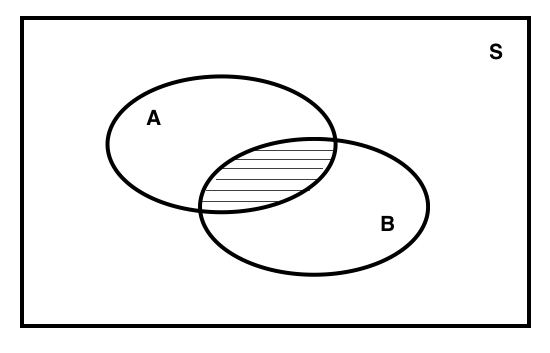
\includegraphics{img/cond1.png}

Example: What is the probability of getting two heads (HH) if we know
that the first coin is H? (1/2)

Example: Suppose we are rolling two dice.

\begin{enumerate}
\def\labelenumi{\alph{enumi}.}
\item
  What is the probability of getting the sum equal to 8?

  \(P(Sum = 8) = P(D_1 = 2, D_2 = 6) + P({3,5}) + P({4,4})*2 + P({5,3}) + P({6,2}) = 6/36 = 1/6\)
\item
  What is the probability of getting the sum more than or equal to 8
  given the first roll is 3?

  \(P(Sum \ge 8 | D_1 = 3) = P({3,5}) + P({3,6}) = 2/6 = 1/3\)
\end{enumerate}

Conditional probability of event A given B, can be defined as
\(P(A|B)=\dfrac{P(A \cap B)}{P(B)}\) if \(P(B) > 0\).

Example: We asked 1000 people, 400 men and 600 women: `Where do you want
to visit this summer? Amsterdam or London?'. The answers are as follows.

\begin{verbatim}
##       Amsterdam London
## Men         150    250
## Women       450    150
\end{verbatim}

\begin{enumerate}
\def\labelenumi{\alph{enumi}.}
\item
  What is the probability of a randomly chosen person is a woman?

  Answer: \(P(W) = (n(W|L) + n(W|P))/n(S) = (150 + 450)/1000 = 0.6\)
\item
  What is the probability of a randomly chosen person chooses to to
  visit Amsterdam?

  Answer: \(P(A) = (n(A|W) + n(A|M))/n(S) = (450 + 150)/1000 = 0.6\)
\item
  What is the probability of a London visitor is a man?

  Answer:
  \(P(M|L) = \dfrac{P(M\cap L)}{P(L)} = \dfrac{n(M\cap L)/n(S)}{n(L)/n(S)} = 250/400 = 0.625\)
\end{enumerate}

\hypertarget{independence}{%
\section{Independence}\label{independence}}

Two events can be independent. It means \(P(A|B) = P(A)\) or
\(P(B|A) = P(B)\).

If the events (\(A_i\)) are independent then
\(P(A_1 \cap A_2 \dots A_k) = P(A_1)P(A_2)\dots P(A_k)\).

Example: Suppose you rolled a die 5 times and they all ended up 4. What
is the probability that, at the 6th time, the die will get 4 again?

Solution: Die rolls are independent events. So outcome of a roll does
not affect the outcome of the other rolls. It is 1/6.

\hypertarget{product-rule}{%
\section{Product rule}\label{product-rule}}

If both \(P(A)>0\) and \(P(B)>0\), then \(P(A\cap B) = P(A)P(B|A)\). We
can also say \(P(A\cap B) = P(B\cap A) = P(B)P(A|B)\)

Example: You draw two cards from a deck. What is the probability that
you get two (A)ces?

Solution: \(P(A \cap B) = 4/52 * 3/52 = 0.00443787\)

Example: You are at a tea shop. There are 10 (W)hite teas, 12 (B)lack
teas and 8 (G)reen teas on the menu. According to the waiter all teas
are equally tasty. You ask the waiter bring a tea but it should not be
green tea. What is the probability that you will get a white tea?

Solution:
\(P(W|G^{\prime}) = P(W \cap G^{\prime})/P(G^{\prime}) = P(W) / P(G^{\prime}) = \dfrac{10/30}{22/30} = 10/22\)

\hypertarget{bayes-rule}{%
\section{Bayes' Rule}\label{bayes-rule}}

\textbf{Theorem of total probability:} Given the events \(B_i\) are
collective parts of the sample space and \(P(B_i) > 0\), then for any
event \(A\), \(P(A) > 0\)

\[P(A) = \sum_i^k P(B_i \cap A) = \sum_i^k P(B_i)P(A|B_i)\]

\textbf{Bayes'rule:} Given the events \(B_i\) are collective parts of
the sample space and \(P(B_i) > 0\), then for any event \(A\),
\(P(A) > 0\)

\[P(B_r|A) = \dfrac{P(B_r|A)}{\sum_i^k P(B_i \cap A)} = \dfrac{P(B_r)P(A|B_r)}{\sum_i^k P(B_i)P(A|B_i)}\]

Example 2.41 from the book: In an assembly plant, there are three
machines \(B_1\), \(B_2\) and \(B_3\). These machines make the 30\%,
45\% and 25\% of the products. 2\%, 3\% and 2\% of their output is known
to be defective. So, what is the probability of getting a defective
product at a random time?

Solution:

Say, event of getting a defective item is A and we want to know
\(P(A)\). \(P(B_i)\) is the probability of a product being manufactured
by machine \(i\). \(P(B_1) = 0.3\), \(P(B_2) = 0.45\),
\(P(B_3) = 0.25\). The defect probabilities given the machine are
\(P(A|B_1) = 0.02\), \(P(A|B_1) = 0.03\), \(P(A|B_1) = 0.02\).

So,
\(P(A) = \sum_{i=1}^3 P(B_i)P(A|B_i) = 0.3*0.02 + 0.45*0.03 + 0.25*0.02 = 0.0245\).

Example 2.42: If the product is defective, what is the probability that
it came from machine 3?

\[P(B_3|A) = \dfrac{P(B_3 \cap A)}{\sum_{i=1}^3 P(B_i)P(A|B_i)} = \dfrac{P(B_3)P(A|B_3)}{\sum_{i=1}^3 P(B_i)P(A|B_i)} = \dfrac{0.25 * 0.02}{0.0245} = 10/49\]

\hypertarget{random-variables-and-distributions}{%
\chapter{Random Variables and
Distributions}\label{random-variables-and-distributions}}

\hypertarget{scales-on-measurement}{%
\section{Scales on Measurement}\label{scales-on-measurement}}

\begin{itemize}
\tightlist
\item
  Nominal scale: These are categorical values that has no relationship
  of order or rank among them. (e.g.~colors, species)
\item
  Ordinal scale: These are categorical values that has relationship of
  order or rank among them (e.g.~military ranks, competiton results).
  Though the relative order has no defined magnitude (e.g.~Champion can
  get 40 points, runner up 39 and third place 30).
\item
  Interval scale: There is a numerical order but the difference can only
  be defined in intervals, \emph{since there is no absolute minimum}. We
  cannot compare in relative values. For instance, we cannot say 10
  degree celsius is twice as hot as 5 degree celsius; what about -5 vs
  +5?
\item
  Ratio scale: Scale with an absolute minimum. (e.g.~If I have 50TL and
  my friend has 100TL, I can say that she has twice the money that I
  have.) Height, weight, age are similar examples.
\end{itemize}

\href{https://en.wikipedia.org/wiki/Level_of_measurement}{See more on
https://en.wikipedia.org/wiki/Level\_of\_measurement}. (p.s. Wikipedia
wasn't banned when I prepared these notes)

\hypertarget{infinity}{%
\section{Infinity}\label{infinity}}

The concept of infinity is very broad. Currently, you just need to keep
the distinction of countable and uncountable infinities in mind.

\begin{itemize}
\tightlist
\item
  Countably infinite: 1, 2, 3, 4, \ldots{} (e.g.~natural numbers,
  integers, \textbf{rational numbers})
\item
  Uncountably infinite: 1, 1.01, 1.001, 1.0001, 1.00001, \ldots{}
  (e.g.~real numbers)
\end{itemize}

How many real numbers are there between 0 and 1?

\hypertarget{descriptive-statistics}{%
\section{Descriptive Statistics}\label{descriptive-statistics}}

Here are brief descriptions of mean (expectation), median, mode,
variance, standard deviation, quantile.

\begin{itemize}
\item
  Mean: \(\bar{X} = \sum_i^N X_i\)
\item
  Median: Let's say \(X_k\) are ordered from smallest to largest and
  there are \(n\) values in the sample. Median(\(X\))\(=X_{(n+1)/2}\) if
  n is odd and (usually)
  Median(\(X\))\(=\dfrac{X_{(n/2)} + X_{(n/2+1)}}{2}\).
\item
  Quantile: On an ordered list of values for quantile (\(\alpha\))
  provides the \((\alpha*n)^{th}\) smallest value of the list. For
  instance, if \(\alpha = 70\% = 0.7\) quantile value is the 7th
  smallest value in a list of 10 values. \(\alpha = 1\) means the
  maximum. Quantile is an important parameter in especially statistics.
\item
  Mode: \(X_k\) with the highest frequency in the sample. In a sample of
  (\(1,2,2,3,4,5\)), \(2\) is the mode.
\item
  Variance: \(V(X) = \dfrac{\sum_i^N (X_i - \bar{X})^2}{n-1}\)
\item
  Standard Deviation:
  \(\sigma(X) = \sqrt{\dfrac{\sum_i^N (X_i - \bar{X})^2}{n-1}}\)
\end{itemize}

\begin{verbatim}
##  [1]  1  9 15 16 16 18 26 31 32 35
\end{verbatim}

\begin{verbatim}
## [1] 19.9
\end{verbatim}

\begin{verbatim}
## [1] 19.9
\end{verbatim}

\begin{verbatim}
## [1] 17
\end{verbatim}

\begin{verbatim}
## 77.77778% 
##        31
\end{verbatim}

\begin{verbatim}
## 0% 
##  1
\end{verbatim}

\begin{verbatim}
## 100% 
##   35
\end{verbatim}

\begin{verbatim}
## numbers
##  1  9 15 16 18 26 31 32 35 
##  1  1  1  2  1  1  1  1  1
\end{verbatim}

\begin{verbatim}
## [1] "16"
\end{verbatim}

\begin{verbatim}
## [1] 118.7667
\end{verbatim}

\begin{verbatim}
## [1] 118.7667
\end{verbatim}

\begin{verbatim}
## [1] 10.89801
\end{verbatim}

\begin{verbatim}
## [1] 10.89801
\end{verbatim}

\hypertarget{random-variables}{%
\section{Random Variables}\label{random-variables}}

A random variable (usually defined with a capital letter or symbol i.e.
\(X\)) is a quantity determined by the outcome of the experiment. Its
realizations are usually symbolized with lowercase letter (\(x\)).

Example: Suppose there are 10 balls in an urn, 5 black and 5 red. Two
balls are randomly drawn from the urn without replacement. Define the
random variable \(X\) as the number of black balls. Then, \(X = x\) can
get the values of 0, 1 and 2. Let's enumerate \(P(X = x)\).

\[P(X = 0) = P(RR) = 5/10 * 4/9 = 2/9\]
\[P(X = 1) = P(BR) + P(RB) = 5/10 + 5/9 + 5/10 * 5/9 = 5/9\]
\[P(X = 2) = P(BB) = 5/10 * 4/9 = 2/9\]

\hypertarget{discrete-random-variables-and-distributions}{%
\section{Discrete Random Variables and
Distributions}\label{discrete-random-variables-and-distributions}}

If a sample space has finite number of possibilities or countably
infinite number of elements, it is called a discrete sample space.
Discrete random variable probabilities are shown as point probabilities
\(P(X = x)\). The probability distribution of discrete random variables
is also called probability mass function (pmf).

\[ P(X=x) = f(x)\] \[\sum_x f(x) = 1\] \[f(x) \ge 0\]

Example: (Same as above) Enumerate the probability distribution.

Solution: Random variable \(X\) can take values (\(x\)) 0, 1 and 2. So
\(f(1) = 2/9\), \(f(2) = 5/9\) and \(f(3) = 2/9\).

\hypertarget{cumulative-distribution-function-cdf}{%
\subsection{Cumulative Distribution Function
(CDF)}\label{cumulative-distribution-function-cdf}}

Cumulative distribution function is a special defined function yielding
the cumulative probability of random variables up to a value. It is
usually symbolised as \(F(x)\)

\[F(x) = P(X \le x) = \sum_{t \le x} f(t)\]
\[F(x) = P(X \le x) = \sum_{\infty} f(t) = 1\]

Example: (Same as above) Enumerate the cdf.

\[F(0) = P(X \le 0) = P(X = 0) = 2/9\]
\[F(1) = P(X \le 1) = P(X = 0) + P(X = 1) = 7/9\]
\[F(2) = P(X \le 2) = P(X = 0) + P(X = 1) + P(X = 2) = 1\]

\hypertarget{continuous-random-variables-and-distributions}{%
\section{Continuous Random Variables and
Distributions}\label{continuous-random-variables-and-distributions}}

If a sample space has uncountably infinite number of possibilities, it
is called a continuous sample space. Continuous random variables'
probabilities are defined in intervals \(P(a < X < b)\). The probability
distribution of continuous random variables is also called probability
density function (pdf).

\[f(x) \ge 0\] \[ P(a < X < b) = f(x) = \int_a^b f(x)dx\]
\[\int_{- \infty}^\infty f(x) = 1\]

Example (from the book): Suppose the probability function of a
continuous distribution \(f(x) = x^2/3\) defined between \(-1 < x < 2\)
and \(0\) everywhere else. Verify that it is a density function
(i.e.~the integral in the defined interval is 1) and calculate
\(P(0 < x < 1)\).

\begin{enumerate}
\def\labelenumi{\alph{enumi}.}
\tightlist
\item
  \(\int_{-1}^2 x^2/3 dx = x^3/9|_{-1}^2 = 8/9 - (-1/9) = 1\). Verified.
\item
  \(\int_{0}^1 x^2/3 dx = x^3/9|_{0}^1 = 1/9 - (0) = 1/9\). Verified.
\end{enumerate}

Cumulative distribution function (CDF) for continuous random variables
is defined with the integral.

\[F(x) = P(X < x) = \int_{- \infty}^a f(x)dx\]

Example: (same as above) Calculate the cdf \(F(3/2)\)

Solution:
\(F(1.5) = \int_{- \infty}^{3/2} f(x) = x^3/9|_{-1}^{3/2} = 3/8 - (-1/9) = 35/72\)

Example: Calculate \(P(X > 1)\).

Solution:
\(P(X > 1) = 1 - P(X < 1) = 1 - F(1) = 1 - \int_{- \infty}^{1} = 1 - ((1/9) - (-1/9)) = 7/9\).

\hypertarget{joint-distribution}{%
\section{Joint Distribution}\label{joint-distribution}}

So far we had distributions with only one random variable. What if we
had more than one random variable in a distribution? It is not that
different from univariate distributions.

\[f(x,y) \ge 0\] \[\sum_x\sum_y f(x,y) = 1\] \[P(X=x,Y=y) = f(x,y)\]

Example (from the book): Two pens are selected at random from a box of 3
blue, 2 red and 3 green pens. Define \(X\) as the number of blue pens
and \(Y\) as the red pens selected. Find

\begin{enumerate}
\def\labelenumi{\alph{enumi}.}
\tightlist
\item
  Joint probability function \(f(x,y)\)
\item
  \(P[(X,Y) \ in A]\) where \(A\) is the region \(\{(x,y)|x+y \le 1\}\).
\end{enumerate}

Solution:

\begin{enumerate}
\def\labelenumi{\alph{enumi}.}
\tightlist
\item
  The possible cases for \((x,y)\) are
  \((0,0),(0,1),(0,2),(1,0),(2,0),(1,1)\). For instance \((0,1)\) is one
  green and one red pen selected. There are a total of 8 pens. Then
  sample space size for two pens selected is \(\binom{8}{2} = 28\).
  There are \(\binom{2}{1}\binom{3}{1} = 6\) ways of selecting 2 pens
  from green and red pens. So the probability is
  \(f(0,1) = P(X=0,Y=1) = 6/28 = 3/14\). It is possible to calculate
  other possible outcomes in a similar way. A generalized formula would
  be as follows.
\end{enumerate}

\[\dfrac{\binom{3}{x}\binom{2}{y}\binom{3}{2-x-y}}{\binom{8}{2}}\]

\begin{enumerate}
\def\labelenumi{\alph{enumi}.}
\setcounter{enumi}{1}
\tightlist
\item
  Possible outcomes satisfying \(A = (x,y) \le 1\) are
  \((0,0),(0,1),(1,0)\). So
  \(P(X+Y \le 1) = P(0,0) + P(0,1) + P(1,0) = 9/14\).
\end{enumerate}

In the continuous case it is similar. It is now called joint probability
density function.

\[f(x,y) \ge 0\] \[\int_x\int_y f(x,y)dxdy = 1\]
\[P(X=x,Y=y) \in A = \int\int_A f(x,y)dxdy\]

Example: (from the book)

A privately owned business operates both a drive in and a walk in
facility. Define \(X\) and \(Y\) as the proportions of using the drive
in and walk in facilities. Suppose the joint density function is
\(f(x,y) = 2/5*(2x+3y)\) where \(0 \le x \le 1\) and \(0 \le y \le 1\)
(0, otherwise).

\begin{enumerate}
\def\labelenumi{\alph{enumi}.}
\tightlist
\item
  Verify it is a distribution function.
\item
  Find \(P[(X,Y)] \in A\), where
  \(A = \{(x,y)|0 < x < 1/2, 1/4 < y < 1/2\}\).
\end{enumerate}

Solution:

\begin{enumerate}
\def\labelenumi{\alph{enumi}.}
\item
  \(\int\int f(x,y)dxdy = \int 2/5*(x^2 + 3xy)dy|_0^1 = \int (2/5 + 6/5*y)dy = 2y/5 + 3/5*y^2 |^1_0 = 2/5 + 3/5 = 1\).
\item
  \(\int_{1/4}^{1/2}\int_0^{1/2} f(x,y)dxdy = \int 2/5*(x^2 + 3xy)dy|_0^{1/2} = \int_{1/4}^{1/2} (1/10 + 3/5*y) dy\),
  \(y/10 + 3y^2/10|_{1/4}^{1/2} = 13/160\).
\end{enumerate}

\hypertarget{marginal-distribution}{%
\section{Marginal Distribution}\label{marginal-distribution}}

In a joint distribution, marginal distribution is the probability
distributions of individual random variables. Define \(g(x)\) and
\(h(y)\) as the marginal distributions of \(X\) and \(Y\).

\[g(x) = \sum_y f(x,y), h(y) = \sum_y f(x,y)\]
\[g(x) = \int_y f(x,y) dy, h(y) = \int_x f(x,y) dx\]

Example: Go back to pen and walk in examples and calculate marginal
probabilities.

\hypertarget{conditional-distribution}{%
\section{Conditional Distribution}\label{conditional-distribution}}

Remember the conditional probability rule \(P(A|B) = P(A \cap B)/P(B)\)
given \(P(B) > 0\). We can define conditional distribution as
\(f(y|x) = f(x,y)/g(x)\), provided \(g(x) > 0\) whether they are
discrete or continuous.

Example: (pen example) Calculate \(P(X=0|Y=1)\)

Solution: We know that \(h(1) = 3/7\). \(f(x=0,y=1) = 3/14\).
\(f(x=0|y=1) = f(x=0,y=1)/h(1) = 1/2\)

\hypertarget{statistical-independence}{%
\section{Statistical Independence}\label{statistical-independence}}

Two random variables distributions are statistically independent if and
only if \(f(x,y) = g(x)h(y)\).

Proof:

\[f(x,y) = f(x|y)h(y)\] \[g(x) = \int f(x,y)dy = \int f(x|y)h(y) dy \]

If \(f(x|y)\) does not depend on \(y\) we can write
\(f(x|y) \int h(y) dy\). \(f(x|y)*1\). Therefore, \(g(x)=f(x|y)\) and
\(f(x,y) = g(x)h(y)\).

Any number of random variables (\(X_1 \dots X_n\)) are statistically
independent if and only if \(f(x_1,\dots,x_n) = f(x_1)\dots f(x_n)\).

\hypertarget{expectation-and-variance}{%
\chapter{Expectation and Variance}\label{expectation-and-variance}}

\emph{This chapter will be improved}

\hypertarget{mathematical-expectation}{%
\section{Mathematical Expectation}\label{mathematical-expectation}}

\[E[X] = \sum x f(x)\] \[E[X] = \int x f(x) dx\]

\hypertarget{variance}{%
\section{Variance}\label{variance}}

\[V(X) = E[X^2] - E[X]^2 \]

\hypertarget{some-discrete-distributions}{%
\chapter{Some Discrete
Distributions}\label{some-discrete-distributions}}

\hypertarget{bernoulli-distribution}{%
\section{Bernoulli Distribution}\label{bernoulli-distribution}}

It can also be called ``single coin toss distribution''. For a single
event with probability of success \(p\) and failure \(q = 1 - p\), the
distribution is called Bernoulli.

\begin{itemize}
\item
  pmf: \(f(x = 0;p) = q\), \(f(x = 1) = p\)
\item
  \(E[X] = 0*(1-p) + 1*p = p\)
\item
  \(V[X] = pq\)
\end{itemize}

Example: Coin Toss

\begin{itemize}
\item
  \(p = 0.5\), \(q = 1 - p = 0.5\)
\item
  pmf: \(f(x = 0) = 0.5\), \(f(x = 1) = 0.5\)
\item
  \(E[X] = 0*(1-0.5) + 1*0.5 = 0.5\)
\item
  \(V(X) = 0.5*0.5 = 0.25\)
\end{itemize}

\hypertarget{binomial-distribution}{%
\section{Binomial Distribution}\label{binomial-distribution}}

Think of multiple Bernoulli trials (e.g.~several coin tosses).

\begin{itemize}
\item
  pmf: \(f(x;p,n) = \binom{n}{x} p^xq^{(n-x)}\)
\item
  \(E[X] = np\)
\item
  \(V(X) = npq\)
\item
  cdf: \(F(X \le x) = \sum_{i=0}^n f(i)\)
\end{itemize}

Example: Multiple Coin Tosses (x5 coins, p = 0.5)

\begin{itemize}
\tightlist
\item
  pmf: \(f(x=3;n=5) = \binom{5}{3} (0.5)^3(1-0.5)^{(5-3)} = 0.3125\)
\end{itemize}

\begin{verbatim}
## [1] 0.3125
\end{verbatim}

\begin{itemize}
\item
  \(E[X] = 5*0.5 = 2.5\)
\item
  \(V(X) = 5*0.5*0.5 = 1.25\)
\item
  cdf: \(F(X \le 3;n=5) = \sum_{i=0}^5 f(i) = 0.8125\)
\end{itemize}

\begin{verbatim}
## [1] 0.8125
\end{verbatim}

\hypertarget{multinomial-distribution}{%
\section{Multinomial Distribution}\label{multinomial-distribution}}

Now suppose there is not one probability (\(p\)) but there are many
probabilities (\(p_1, p_2, \dots, p_k\)).

\begin{itemize}
\item
  pmf:
  \(f(x_1, \dots , x_k;p_1, \dots, p_k;n) = \binom{n}{x_1, \dots , x_k} p_1^{x_1}*\dots *p_k^{x_k}\)

  where \(\binom{n}{x_1, \dots , x_k} = \dfrac{n!}{x_1! \dots x_k!}\),
  \(\sum_i^k x_i = n\) and \(\sum_i^k p_i = 1\).
\end{itemize}

Example: Customers of a coffee shop prefer Turkish coffee with
probability 0.4, espresso 0.25 and filter coffee 0.35. What is the
probability that out of the first 10 customers, 3 will prefer Turkish
coffee, 5 will prefer espresso and 2 will prefer filter coffee?

\(f(3,5,2;0.4,0.25,0.35;10) = \binom{10}{3,5,2} * 0.4^3 * 0.25^5 * 0.35^10 = 4.3 * 10^{-6} = 0.0193\)

\begin{verbatim}
## [1] 0.01929375
\end{verbatim}

\begin{verbatim}
## [1] 0.01929375
\end{verbatim}

Binomial distribution is a special case of multinomial distribution.

\hypertarget{hypergeometric-distribution}{%
\section{Hypergeometric
Distribution}\label{hypergeometric-distribution}}

Hypergeometric distribution can be used in case the sample is divided in
two such as defective/nondefective, white/black, Ankara/Istanbul.
Suppose there are a total of \(N\) items, \(k\) of them are from group 1
and \(N-k\) of them are from group 2. We want to know the probability of
getting \(x\) items from group 1 and \(n-k\) items from group 2.

\begin{itemize}
\item
  pmf:
  \(f(x,n;k,N) = \dfrac{\binom{k}{x}\binom{N-k}{n-x}}{\binom{N}{n}}\)
\item
  \(E[X] = \dfrac{nk}{N}\)
\item
  \(V[X] = \dfrac{N-n}{N-1}*n*\dfrac{k}{N}*(1-\dfrac{k}{N})\)
\end{itemize}

Example: Suppose we have a group of 20 people, 12 from Istanbul and 8
from Ankara. If we randomly select 5 people from it what is the
probability that 1 of them is from Ankara and 4 of them from Istanbul.

\(f(1,5;8,20) = \dfrac{\binom{8}{1}\binom{20-8}{5-1}}{\binom{20}{5}} = 0.256\)

\begin{verbatim}
## [1] 0.255418
\end{verbatim}

\begin{verbatim}
## [1] 0.255418
\end{verbatim}

\hypertarget{negative-binomial-distribution}{%
\section{Negative Binomial
Distribution}\label{negative-binomial-distribution}}

Negative Binomial distribution answers the question ``What is the
probability that k-th success occurs in n trials?''. Differently from
the binomial case, we fix the last attempt as success.

\begin{itemize}
\tightlist
\item
  pmf: \(f(x;p,n) = \binom{n-1}{x-1} p^xq^{(n-x)}\)
\end{itemize}

Example: Suppose I'm repeatedly tossing coins. What is the probability
that 3rd Heads come in the 5th toss?

\(f(3;0.5,5) = \binom{5-1}{3-1} 0.5^30.5^{(5-3)} = 0.1875\)

\begin{verbatim}
## [1] 0.1875
\end{verbatim}

\begin{verbatim}
## [1] 0.1875
\end{verbatim}

\begin{verbatim}
## [1] 0.1875
\end{verbatim}

\hypertarget{geometric-distribution}{%
\section{Geometric Distribution}\label{geometric-distribution}}

Geometric distribution answers ``What is the probability that first
success comes in the n-th trial?''

\begin{itemize}
\item
  pmf: \(f(x;p,n) = q^{(n-1)}p\)
\item
  \(E[X] = 1/p\)
\item
  \(V[X] = \dfrac{1-p}{p^2}\)
\end{itemize}

\hypertarget{poisson-distribution}{%
\section{Poisson Distribution}\label{poisson-distribution}}

Poisson distribution is widely used to represent occurences in an
interval, mostly time but sometimes area. Examples include arrivals to
queues in a day, number of breakdowns in a machine in a year, typos in a
letter, oil reserve in a region.

\hypertarget{binomial-approximation-to-poisson-distribution}{%
\subsection{Binomial Approximation to Poisson
Distribution}\label{binomial-approximation-to-poisson-distribution}}

We know from binomial distribution that \(k\) occurences in \(n\) trials
with probability \(p\) has the following function.

\[P\{X = k\} = \binom{n}{k} p^k (1-p)^{n-k} = \dfrac{n!}{(n-k)!k!} p^k (1-p)^{n-k}\]

and expected value is \(E[X] = np\). Now define \(\lambda = np\).

\begin{align*}
P\{X = k\} =& \dfrac{n!}{(n-k)!k!} \left(\dfrac{\lambda}{n}\right)^k \left(1-\left(\dfrac{\lambda}{n}\right)\right)^{n-k} \\
           =& \dfrac{n (n-1) \dots (n-k+1)}{n^k} \left(\dfrac{\lambda^k}{k!}\right) \dfrac{(1-\dfrac{\lambda}{n})^n}{(1-\dfrac{\lambda}{n})^k}
\end{align*}

For very large \(n\) and very small \(p\) the resulting pdf becomes
\(\dfrac{\lambda^k e^{-\lambda}}{k!}\).

\hypertarget{properties-of-poisson-distribution}{%
\subsection{Properties of Poisson
Distribution}\label{properties-of-poisson-distribution}}

\begin{itemize}
\item
  PMF: \(P\{X = k\} = \dfrac{\lambda^k e^{-\lambda}}{k!}\)
\item
  CDF:
  \(P\{X \le k\} = \sum_{i=0}^k \dfrac{\lambda^i e^{-\lambda}}{i!}\)
\item
  \(E[X] = \lambda (due to \sum_{i=0}^\infty\dfrac{x^i}{i!} = e^x)\)
\item
  \(V(X) = \lambda\)
\end{itemize}

Rate parameter \(\lambda\) can also be defined as \(\lambda t\), \(t\)
being the scale parameter. For instance, let arrivals in 30 minutes
interval be \(\lambda t_{30} = 4\). If we would want to work on hourly
intervals, we should simply rescale, \(\lambda t_{60} = 8\).

\hypertarget{chapter-questions}{%
\section{Chapter Questions}\label{chapter-questions}}

\begin{enumerate}
\def\labelenumi{\arabic{enumi}.}
\item
  A boutique shop offers three types of breads; olive, rye and white.
  15\% of its customers buy olive bread, 55\% rye bread and the rest
  white bread. What is the probability that the first 10 customers of
  the shop buys 2 olive, 5 rye and 3 white bread?

  \emph{Solution:} Multinomial distribution.

  \[\binom{10}{2,5,3} 0.15^2 * 0.55^5 * 0.3^3 = 0.0770478\]

\begin{verbatim}
## [1] 0.0770478
\end{verbatim}
\item
  An urn contains 32 balls; 18 red, 14 white. If I take 8 balls randomly
  from the urn, what is the probability of getting 4 red balls?

  \emph{Solution:} Hypergeometric distribution.

  \[\dfrac{\binom{18}{4}\binom{14}{4}}{\binom{32}{8}} = 0.2912125\]

\begin{verbatim}
## [1] 0.2912125
\end{verbatim}
\item
  A UNICEF activist asks bypassers to contribute to their efforts. Each
  of her attempts has a 10\% chance of success. What is the probability
  that she got the first contribution at the 10th attempt?

  \emph{Solution:} Geometric distribution.

  \[ (0.9)^9 * (0.1) = 0.03874205\]

\begin{verbatim}
## [1] 0.03874205
\end{verbatim}
\item
  Suppose there are 10 cards in a deck numbered from 1 to 10. If I draw
  four cards out of the deck without putting them back, what is the
  probability that they are in increasing order (e.g.~3-4-5-8)?

  \emph{Solution}: Increasing order is a special order. There is only
  one decreasing order in every permutation set. For instance

  \[8-5-4-3\] \[8-5-3-4\] \[8-4-5-3\] \[4-5-3-8\] \[\dots\]
  \[**3-4-5-8**\]

  So, the answer is \(1/(4!) = 1/24\).
\item
  A tennis player has the probability of 0.15 to ace a serve (i.e.~he
  serves and gets the point without the opponent touching the ball) at
  each shot. His trainer challenged him that he will pay the square of
  the aces he makes out of 10 serves (e.g.~if he serves 8 aces out of
  10, the trainer pays him \(8^2 = 64TL\)). But, if he serves less than
  or equal to 6 aces, the player should pay the trainer 5 TL for each
  ace he missed (e.g.~4 aces 6 misses, player pays up 6*5 = 30TL).

  \begin{enumerate}
  \def\labelenumii{\alph{enumii})}
  \tightlist
  \item
    What is the maximum amount of money he can get?
  \item
    What is the expected earnings of the player?
  \item
    What is the variance of his earnings?
  \end{enumerate}

  \emph{Solution:}

  \begin{enumerate}
  \def\labelenumii{\alph{enumii})}
  \item
    10 out of 10 means 10\^{}2 = 100.
  \item
    \(g(X = x) = x^2\) if \(x \geq 7\), \(-x\) else,
    \(f(g(X) = x^2) = f(X = x) = \binom{10}{x} 0.15^x * 0.85^(10-k)\),
    so \(E[g(x)] = \sum_{i=0}^10 g(x)f(x)\).

    So
    \(49 * \binom{10}{7} 0.15^7 * 0.85^3 + 64 * \binom{10}{8} 0.15^8 * 0.85^2 + 81 * \binom{10}{9} 0.15^9 * 0.85 + 100 * (0.15)^10\)
    \(-20 * \binom{10}{6} 0.15^6 * 0.85^4 -25 * \binom{10}{5} 0.15^5 * 0.85^5 - 30 * \binom{10}{4} 0.15^4 * 0.85^6 - 35 * \binom{10}{3} 0.15^3 * 0.85^7 - 40 * \binom{10}{2} 0.15^2 * 0.85^8 - 45 * \binom{10}{1} 0.15^1 * 0.85^9 - 50 * 0.85^10 = -42.5TL\).
  \end{enumerate}

\begin{verbatim}
## [1] -42.4913
\end{verbatim}

  \begin{enumerate}
  \def\labelenumii{\alph{enumii})}
  \setcounter{enumii}{2}
  \tightlist
  \item
    \(V(X) = E[X^2] - (E[X])^2\). We know that \(E[X] = -42.5\), then
    \((E[X])^2 = 1805.51\). Also \(E[X^2] = 1838.434\) and
    \(V(X) = 32.92\).
  \end{enumerate}

\begin{verbatim}
## [1] 32.92423
\end{verbatim}
\item
  Suppose a machine has a probability of failure 0.001 per hour. What is
  the probability that the machine had failed at least three times
  within 2000 hours.

  \emph{Binomial solution}

  \begin{align*}
   P\{X \ge 3\} &= 1 - \binom{2000}{0} 0.001^0 0.999^{750} - \binom{2000}{1} 0.001^1 0.999^{749} - \binom{2000}{2} 0.001^2 0.999^{748} \\
   &= 0.3233236
   \end{align*}

\begin{verbatim}
## [1] 0.3233236
\end{verbatim}

  \emph{Poisson solution}

  \begin{align*}
   \lambda &= np = 2000*0.001 = 2 \\
   P\{X \ge 3\} &= 1 - \dfrac{e^{-2}2^0}{0!} - \dfrac{e^{-2}2^1}{1!} - \dfrac{e^{-2}2^2}{2!} \\
       &= 0.3233236
   \end{align*}

\begin{verbatim}
## [1] 0.3233236
\end{verbatim}
\item
  People arrive at a bank with rate \(\lambda = 5\) every 10 minutes.
  What is the probability that 10 people arrive in 30 minutes?

  \[\lambda t_{10} = 5\]

  \[\lambda^\prime = \lambda t_{30} = 15 \]

  \[P\{X = 10, t=30\} = \dfrac{e^{-15}15^{10}}{10!} =  0.049\]

\begin{verbatim}
## [1] 0.04861075
\end{verbatim}
\item
  A machine breaks down with a poisson rate of \(\lambda = 10\) per
  year. A new method is tried to reduce the failure rate to
  \(\lambda = 3\), but there is a 50\% chance that it won't work. If the
  method is tried and the machine fails only 3 times that year, what is
  the probability that the method worked on the machine?

  \begin{align*}
   P\{Works | X = 3\}  &= \dfrac{P\{Works and X = 3\}}{P\{X = 3\}} \\~\\
   P\{Works\} &= 0.5\\~\\
   P\{Works and X = 3\} &= 0.5 * \dfrac{e^{-3}3^3}{3!} = 0.1120209\\~\\
   P\{X = 3\} &= P\{Works and X = 3\} + P\{Doesn't\ Work and X = 3\} = 0.5 * \dfrac{e^{-3}3^3}{3!} + 0.5 * \dfrac{e^{-10}10^3}{3!} \\
   &= 0.96733
   \end{align*}

\begin{verbatim}
## [1] 0.96733
\end{verbatim}
\end{enumerate}

\hypertarget{exercise-questions}{%
\chapter{Exercise Questions}\label{exercise-questions}}

\textbf{Question 1}

How many ways are there to arrange ``ECONOMETRICS''.

Solution: There 12 characters, 5 vowels 7 consonants. 2 Cs, 2 Es and 2
Os.

\begin{enumerate}
\def\labelenumi{\alph{enumi})}
\tightlist
\item
  In any order.
\end{enumerate}

Solution: \(\dfrac{12!}{2!2!2!}\).

\begin{enumerate}
\def\labelenumi{\alph{enumi})}
\setcounter{enumi}{1}
\tightlist
\item
  Vowels together.
\end{enumerate}

Solution: Add one representative letter to consonants to denote vowels
as a single letter. \(\dfrac{8!}{2!}\dfrac{5!}{2!2!}\).

\begin{enumerate}
\def\labelenumi{\alph{enumi})}
\setcounter{enumi}{2}
\tightlist
\item
  No consecutive vowels.
\end{enumerate}

Solution: \(\dfrac{7!}{2!}\dfrac{8!}{(8-5)!2!2!}\)

\textbf{Question 2}

7 people from Istanbul (suppose names A-B-C-D-E-F-G) and 7 people from
Ankara (M-N-O-P-Q-R-S) will sit around a round table.

\begin{enumerate}
\def\labelenumi{\alph{enumi})}
\tightlist
\item
  In how many different ways can they sit around the table?
\end{enumerate}

Solution: \((14-1)! = 13!\)

\begin{enumerate}
\def\labelenumi{\alph{enumi})}
\setcounter{enumi}{1}
\tightlist
\item
  Same as (a) but no two people from Ankara should sit together.
\end{enumerate}

Solution: Fix one from Istanbul to a position. \((7-1)!(7)!\)

\begin{enumerate}
\def\labelenumi{\alph{enumi})}
\setcounter{enumi}{2}
\tightlist
\item
  Same as (a) but all the people from Istanbul should sit together.
\end{enumerate}

Solution: Suppose there are 8 people from Ankara, 1 reserved for
Istanbul group and Istanbul people have their own permutation within.
\((8-1)!7!\)

\textbf{Question 3}

You roll a die once, and assume the number your rolled is X. Then
continue rolling the die until you either match or exceed X. What is the
expected number of additional rolls?

Solution:

\[E[n|X_1=i] = 1/P(X_2 \ge i| X_1 = i) = 6/(6-i+1)\]

\[\sum_{i=1}^6 = 6/(6-i+1) * P(X=i) = 2.45\]

\textbf{Question 4}

In a three dice roll, if at least two dice have the same number
(e.g.~5-5-4 or 3-3-3) you win.

\begin{enumerate}
\def\labelenumi{\alph{enumi})}
\tightlist
\item
  What is the probability that you win at least three times in a 30
  rolls game?
\end{enumerate}

Solution: All combinations \(N = 6^3 = 216\). Non repeating permutations
\(n_{lose} = \dfrac{6!}{3!} = 120\). Probability of win is
\(1 - \dfrac{n_lose}{N} = 0.444\). Probability of winning at least 3
times is
\[P(X \ge 3| T = 30) = 1 - P(X = 0|T=30) - P(X = 1|T=30) - P(X=2|T=30)\]
\[P(X \ge 3| T = 30) = 1 - 0.9999933\]

\begin{enumerate}
\def\labelenumi{\alph{enumi})}
\setcounter{enumi}{1}
\tightlist
\item
  What is the expected number and variance of the number of wins?
\end{enumerate}

\[E[X] = np = 30*(0.444) = 13.33\]
\[V[X] = np(1-p) = 30*(0.444)*(1-0.444) = 7.407407\]

\textbf{Question 5}

In a Go game, a player that wins three games out of five is the winner.
Suppose the artificial intelligence Alpha Go has probability 0.65 of
winning against the World's (Human) Go Champion. What is the probability
that Alpha Go wins the game at the 4th game?

Solution: AI should win 2 games in the first 3 and win the 4th game.
\(\binom{3}{2}(0.65)^2(0.35)(0.65) = 0.289\)

\textbf{Question 6}

An egg basket contains 8 eggs, 4 of which are broken. 3 eggs are
selected to make an omelette.

\begin{enumerate}
\def\labelenumi{\alph{enumi})}
\tightlist
\item
  What is the probability that all 3 eggs are intact?
\end{enumerate}

Solution: \(\dfrac{\binom{4}{3}}{\binom{8}{3}} = 0.0714\)

\begin{enumerate}
\def\labelenumi{\alph{enumi})}
\setcounter{enumi}{1}
\tightlist
\item
  What is the probability that the 2nd broken egg is the 3rd egg?
\end{enumerate}

Solution: Probability of getting 1 intact and 1 broken egg
\(\dfrac{\binom{4}{1}\binom{4}{1}}{\binom{8}{2}} = 0.571\). At 3rd egg
there should be 3 intact and 3 broken eggs remaining, so getting the 3rd
broken egg is 1/2. Final probability is \(0.286\).

\textbf{Question 7}

Nejat is a film critic and he will attend to IKSV Film Festival between
April 5-15. Nejat likes a movie with probability 0.6 if the genre of the
movie is mystery. For other genres, he likes the movie with probability
0.4. There will be 40 movies during the festival, 10 of which are
mystery.

\begin{enumerate}
\def\labelenumi{\alph{enumi})}
\tightlist
\item
  What is the probability that Nejat will like a randomly selected
  movie?
\end{enumerate}

Solution: (L)ike, (D)islike, (M)ystery, (O)ther.
\(P(M) = 10/40 = 0.25\).
\[P(L) = P(L|M)P(M) + P(L|O)P(O) = 0.6*0.25 + 0.4*0.75 = 0.45\]

\begin{enumerate}
\def\labelenumi{\alph{enumi})}
\setcounter{enumi}{1}
\tightlist
\item
  Suppose Nejat did not like the film. What is the probability that the
  selected movie is a non-mystery film?
\end{enumerate}

Solution:
\(P(O|D) = \dfrac{P(D|O)P(O)}{P(D)} = \dfrac{P(D|O)P(O)}{1-P(L)} = 0.6*0.75/0.55 = 0.818\)

\textbf{Question 8}

A student applies for internships to 11 companies. She has a 0.6
probability to get an offer for an internship.

\begin{enumerate}
\def\labelenumi{\alph{enumi})}
\tightlist
\item
  What is the probability that she will get offers from at least 4
  companies?
\end{enumerate}

Solution:
\(P(X \ge 4) = \sum_{i=4}^{11} \binom{8}{i} (0.6)^i(0.4)^{n-i} = 0.97\)

\begin{enumerate}
\def\labelenumi{\alph{enumi})}
\setcounter{enumi}{1}
\tightlist
\item
  What is the probability that she gets her fourth offer at the seventh
  application?
\end{enumerate}

Solution: \(\binom{6}{3} (0.6)^3(0.4)^{3}(0.6) = 0.166\)

\begin{enumerate}
\def\labelenumi{\alph{enumi})}
\setcounter{enumi}{2}
\tightlist
\item
  What is the expected value and variance of the applications?
\end{enumerate}

Solution: \(E[X] = np = 11*0.6 = 6.6\),
\(V(X) = np(1-p) = 11*0.6*0.4 = 2.64\).

\textbf{Question 9}

A steakhouse serves (C)hateaubriand, (K)obe Beef Tenderloin and
(T)-Bone. Customers order C with probability 0.35, K w.p. 0.2 and T w.p.
0.45.

\begin{enumerate}
\def\labelenumi{\alph{enumi})}
\tightlist
\item
  12 customers arrive. What is the probability that 4 of them order C, 3
  order K and 5 order T?
\end{enumerate}

Solution: \(\binom{12}{4,3,5}(0.35)^4(0.2)^3(0.45)^5 = 0.0614\).

\begin{enumerate}
\def\labelenumi{\alph{enumi})}
\setcounter{enumi}{1}
\tightlist
\item
  Suppose C sells for 90TL, K for 150TL and T for 120TL. If 100
  customers are served that day, what is the expected revenue?
\end{enumerate}

Solution: \(100*(90*0.35 + 150*0.2 + 120*0.45) = 11550TL\).

\textbf{Question 10}

An international student group will select a committee of 4 people at
random. There are 7 Turkish, 6 Greek, 4 Italian and 5 Irish students in
the group.

\begin{enumerate}
\def\labelenumi{\alph{enumi})}
\tightlist
\item
  What is the probability that all countries are represented?
\end{enumerate}

Solution: Total number students is 22.
\(\dfrac{7*6*4*5}{\binom{22}{4}} = 0.1148325\)

\begin{enumerate}
\def\labelenumi{\alph{enumi})}
\setcounter{enumi}{1}
\tightlist
\item
  If the committee consisted of 5 people what would be the probability
  of (a)?
\end{enumerate}

Solution:
\(\dfrac{7*6*4*\binom{5}{2} + 7*6*5*\binom{4}{2} + 7*5*4*\binom{6}{2} + 6*5*4*\binom{7}{2}}{\binom{22}{4}} = 0.287\)

\textbf{Question 11}

There are 3 balls in an urn, each of them is either (B)lack or (W)hite.
At each step \(i\), a ball is drawn from the urn randomly and another
ball is thrown the urn with equal probability for both colors. So there
are three balls at the end of each step. Let \(X_i\) be the number of
White balls at time \(i\). We know that at step 0, there are two white
balls and one black ball in the urn (i.e. \(X_0 = 2\)). Calculate the
following.

a) \(P(X_1 = 2 | X_0 = 2)\)

b) \(P(X_2 = 1 | X_0 = 2)\)

Now consider that the process is switched. First, a ball is thrown at
random inside the urn then a ball is drawn from the urn. Again at step
0, there are two white balls and one black ball (i.e. \(X_0 = 2\)).
Calculate the following.

c) \(P(X_1 = 1 | X_0 = 2)\)

d) \(P(X_2 = 2 | X_0 = 2)\)

Solution: Define \(Y_i\) as the ball drawn the urn and \(Z_i\) as the
ball added at stage \(i\). Probabilities of \(Z\) will always be the
same. \(P(Z_i=W) = P(Z_i=B) = 0.5\). For a and b, probabilities of
\(Y_i\) is dependent only on \(X_{i-1}\). But, for c and d, \(Y\)
depends on both \(X_{i-1}\) and \(Z_i\).

a)
\(P(X_1 = 2 | X_0 = 2) = P(Y_1 = W|X_0=2)P(Z_1 = W) + P(Y_1 = B|X_0=2)P(Z_1 = B) = 2/3*1/2 + 1/3*1/2 = 1/2\).
b)
\(P(X_2 = 1|X_0=2) = P(X_2 = 1| X_1 = 2, X_0=2) + P(X_2 = 1| X_1 = 1,X_0=2) = P(X_2=1|X_1=2)P(X_1=2|X_0=2) + P(X_2=1|X_1=1)P(X_1=1|X_0=2)\).
We can say that P(X\_i = x\_i\textbar{}X\_\{i-1\} = x\_\{i-1\}) is equal
for all \(i\). So
\(P(X_2=1|X_1=2)P(X_1=2|X_0=2) + P(X_2=1|X_1=1)P(X_1=1|X_0=2) = P(X_1=1|X_0=2)P(X_1=2|X_0=2) + P(X_1=1|X_0=1)P(X_1=1|X_0=2) = P(X_1=1|X_0=2)(P(X_1=2|X_0=2)+P(X_1=1|X_0=1))\).
Then \(P(X_1=1|X_0=2) = P(Y_1=W|X_0=2)P(Z_1=B) = 2/3*1/2 = 1/3\).
\(P(X_1=1|X_0=1) = P(Y_1 = W|X_0=1)P(Z_1 = W) + P(Y_1 = B|X_0=1)P(Z_1 = B) = 1/3*1/2 + 2/3*1/2 = 1/2\).

So, \(P(X_1 = 2 | X_0 = 2) = 1/3*(1/2 + 1/2) = 1/3\).

c) Similar but this time \(Z_i\) is more important.
\(P(X_1 = 1 | X_0 = 2) = P(Z_1 = B)P(Y_1 = B|X_0=2,Z_1=B) = 1/2*1/2=1/4\).

d)
\(P(X_2 = 2 | X_0 = 2) = P(X_2 = 2 | X_1 = 2)P(X_1 = 2 | X_0 = 2) + P(X_2 = 2 | X_1 = 1)P(X_1 = 1 | X_0 = 2) + P(X_2 = 2 | X_1 = 3)P(X_1 = 3 | X_0 = 2)\).
Let's rephrase
\(P(X_1 = 2 | X_0 = 2)^2 + P(X_1 = 2 | X_0 = 1)P(X_1 = 1 | X_0 = 2) + P(X_1 = 2 | X_0 = 3)P(X_1 = 3 | X_0 = 2)\).
\(P(X_1 = 2 | X_0 = 2) = 1/2*3/4 + 1/2*1/4 = 1/2\).
\(P(X_1 = 2|X_0 = 1) = 1/2*1/2 = 1/4\).
\(P(X_1 = 3|X_0 = 2) = 1/2*1/4 = 1/8\).
\(P(X_1 = 2|X_0 = 3) = 1/2*3/4 = 3/8\).

\[(1/2)^2 + 1/4 * 1/4 + 1/8*3/8 = 23/64\]

\textbf{Question 12}

Calculate the number of permutations of the word ``SUCCESSFUL'' with
vowels together.

Solution: 3S, 2C, 1L, 1F, 2U and 1F. 7 consonants, 3 vowels.
\(\dfrac{(7+1)!}{3!2!}\dfrac{3!}{2!}=10800\).

\textbf{Question 13}

10 students enter the cafeteria. There are three different meal choices;
red meat, vegeterian and fish. A student prefers red meat with 50\%
probability, vegeterian 20\% and fish 30\%. What is the probability
that, of this group of 10, 4 students prefer eat red meat, 3 students
prefer vegeterian and 3 students prefer fish?

Solution: Multinomial Distribution
\(\binom{10}{4,3,3}(0.5)^4(0.2)^3(0.3)^3 = 0.0567\)

\textbf{Question 14}

Three students are going to start an internship on January. There are
five internship posts on the department website. Each has to apply to
only one internship. What is the probability that none of the students
apply to the same internship?

Solution: Similar to birthday problem. \(\dfrac{5!}{2!}/5^3 = 0.48\).

\textbf{Question 15}

Baran is an activist who raises funds for UNICEF on the street. 80\% of
people walking by stops when Baran asks to tell about UNICEF. 50\% of
those who stop donates 10TL to UNICEF. What is the expected amount of
donations if Baran tried to reach 15 people that day.

Solution: P(Donation) = P(Stop)P(Donation\textbar{}Stop) = 0.8*0.5 =
0.4. Expectation of binomial distribution np = 15*0.4 = 60.

\textbf{Question 16}

Merve is an aspiring singer. She has 25\% chance to be offered to sing
at a concert, if she applies. She applied to 8 concerts for the next
season. What is the probability that she got at least 2 offers?

Solution: P(Reject) = 0.75.
\(P(X \ge 2) = 1 - P(0) - P(1) = 1 - (0.75^8 + 8*0.75^7*0.25) = 0.64\)

\textbf{Question 17}

Bureau of Statistics provide you with the following information. 40\% of
Architects, 60\% of Engineers and 30\% of Lawyers make more than 5000TL
per month in the first two years of their career. Of those interested in
these occupations 20\% choose Architecture, 50\% choose Engineering and,
30\% choose Law.

a) What is the probability that a randomly selected person from these
careers make less than 5000TL per month in the first two years of
his/her career?

b) If a person makes more than 5000TL, what is the probability that
he/she is an Architect?

Solution: Define \(W\) as making more than 5000TL, \(W^c\) as less and
(A) as choosing Architecture career, (E) Engineering and (L) Law.

a) \(P(W^c|A) = 1 - P(W|A) = 0.6\), \(P(W^c|E) = 1 - P(W|E) = 0.4\),
\(P(W^c|L) = 1 - P(W|L) = 0.7\).
\(P(W^c) = P(A)P(W^c|A)+P(E)P(W^c|E)+P(L)P(W^c|L) = 0.2*0.6+0.5*0.4+0.3*0.7 = 0.53\).

b) \(P(A|W) = P(A \cap W)/P(W)\).
\(P(A \cap W) = P(A)P(W|A) = 0.2*0.4 = 0.08\).
\(P(W) = 1 - P(W^c) = 0.47\). \(P(A|W) = 0.08/0.47 = 0.17\).

\textbf{Question 18}

Let \(X\) and \(Y\) be the random variables and \(f(x,y)\) is the
probability density function of the joint distribution. Suppose
\(f(x,y)\) is defined as \(k(2x^2 + y)\) if \(0<x<2\) and \(0<y<1\) (0
otherwise).

a) Find \(k\).

b) Find the marginal distribution of \(y\) (\(h(y)\)) and \(h(y<0.5)\).

c) Find the conditional distribution of \(f(y|x)\).

Solution:

a)
\(\int^1_0 \int^2_0 k(2x^2 + y) dx dy = \int^1_0 k((2/3)*x^3 + xy)dy|^2_0 = \int^1_0 k(16/3+2y) dy\).
(This is also \(h(y)\) if \(k\) is known.)
\(k(16y/3+y^2)|^1_0 = k(19/3)\). In order to be a distribution it should
be equal to 1. So \(k = 3/19\).

b) As given in (a) \(h(y) = 3/19(16/3+2y)\). So
\(h(y<0.5) = \int^{0.5}_0 3/19(16/3+2y) dy = 3/19(16y/3+y^2)|^{0.5}_0 = 3/19(8/3 + 1/4) = 3/19*33/12 = 0.43\)

c) We need to find
\(g(x) = \int^1_0 3/19(2x^2 + y)dy = 3/19(2x^2 + 1/2)\).
\(f(y|x) = f(x,y)/g(x) = \dfrac{3/19(2x^2+y)}{3/19(2x^2 + 1/2)} = \dfrac{4x^2 + 2y}{4x^2 + 1}\).

\hypertarget{some-continuous-distributions}{%
\chapter{Some Continuous
Distributions}\label{some-continuous-distributions}}

So far we had only seen discrete distributions which only specific
values have positive probability values. Now we are going to see
continuous variables where each real value defined in the domain of the
distribution has a positive probability.

In this class we are going to see uniform, exponential, normal, gamma
and weibull distributions. Of those, we will see uniform, exponential
and normal distributions in detail.

\hypertarget{uniform-distribution}{%
\section{Uniform Distribution}\label{uniform-distribution}}

Given an interval \([a,b]\), each value within the interval has equal
probability in uniform distribution.

\[X \sim U[a,b]\]

\begin{itemize}
\item
  Density: \(f(X) = \dfrac{1}{b-a}\)
\item
  CDF: \(F(X \le x) = \dfrac{x-a}{b-a}\)
\item
  \(E[X] = (b+a)/2\)
\item
  \(V(X) = 1/12(b-a)^2\)
\end{itemize}

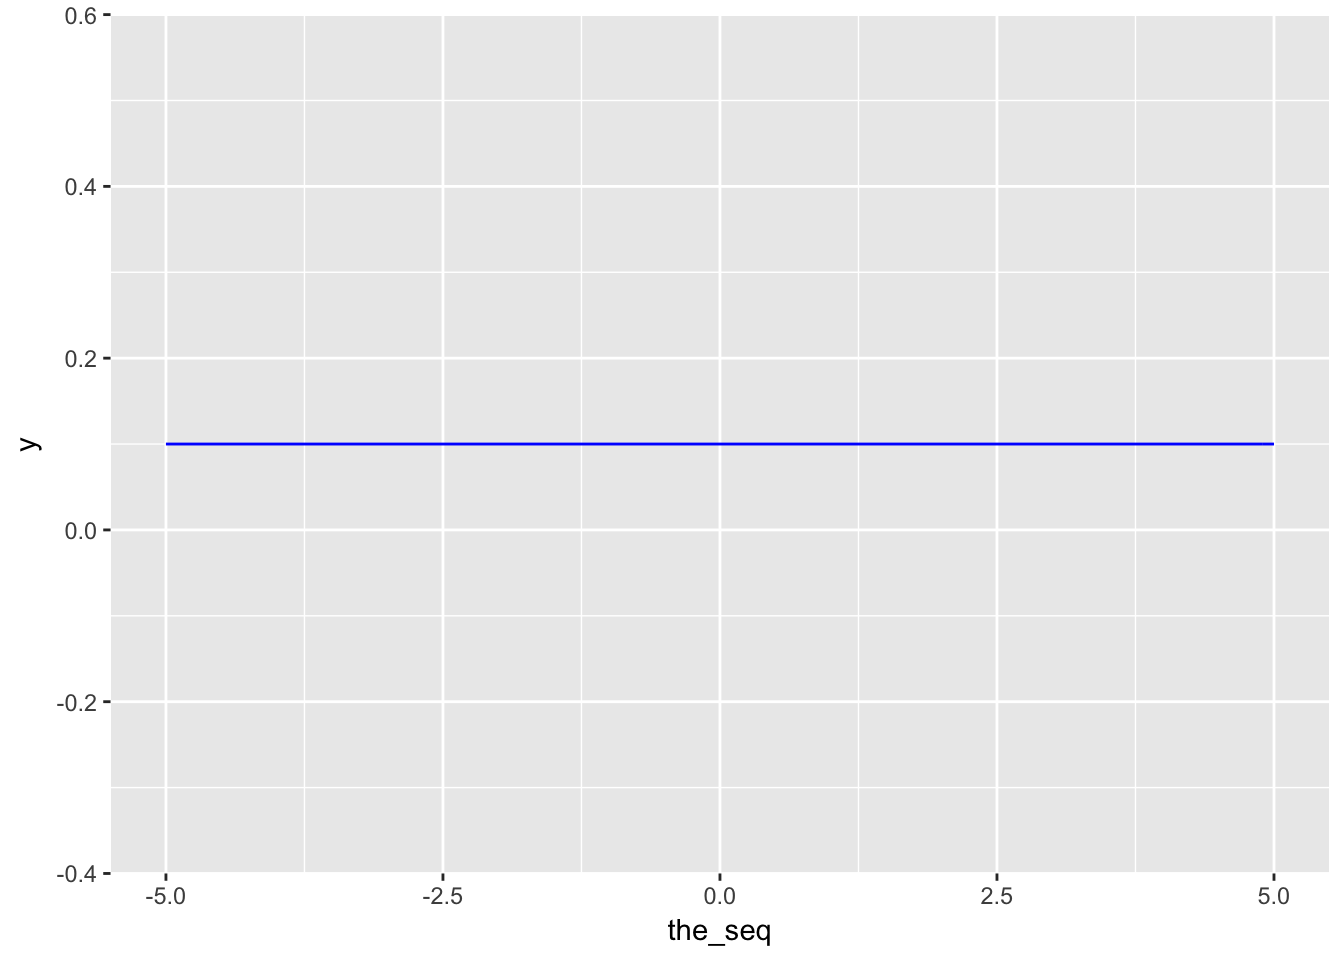
\includegraphics{book-of-prob_files/figure-latex/unif-1.pdf}

Example: Suppose there is a lecture that can end anytime between 11:00
and 13:00. What is the probability that it ends before 12:30?

Solution: There are 120 minutes betweeen 11:00 (a) and 13:00 (b) and 90
minutes between 11:00 (a) and 12:30 (x).

\[P(X \le 90) = 90/120 = 3/4\]

\hypertarget{exponential-distribution}{%
\section{Exponential Distribution}\label{exponential-distribution}}

Exponential distribution is generally used to measure time before an
event happens. Common examples are component (i.e.~light bulb) lifetime
and job processing (i.e.~queue serving). It is closely related to
Poisson distribution. While Poisson is used to estimate number of events
in a given time period, Exponential distribution estimates the time of
an event.

\begin{itemize}
\item
  Density: \(f(X) = \lambda e^{-\lambda x}\)
\item
  CDF: \(F(X \le x) = 1 - e^{-\lambda x}\)
\item
  \(E[X] = 1/\lambda\)
\item
  \(V(X) = 1/\lambda^2\)
\end{itemize}

Exponential distribution has memoryless property.

\[P(X > t + s | X > t) = \dfrac{P(X > t + s)}{P(X > t)} = \dfrac{e^{-\lambda (t+s)}}{e^{-\lambda t}} = e^{-\lambda s}\]

Note: Exponential distribution is frequently used in maintenance themed
questions (e.g. ``A machine breaks down\ldots{}''). Though, memoryless
property in exponential distribution might seem a bit off as it kind of
assumes replenished starting point and no ``wear and tear effect''.
Don't forget these are mathematical questions and applications might
differ.

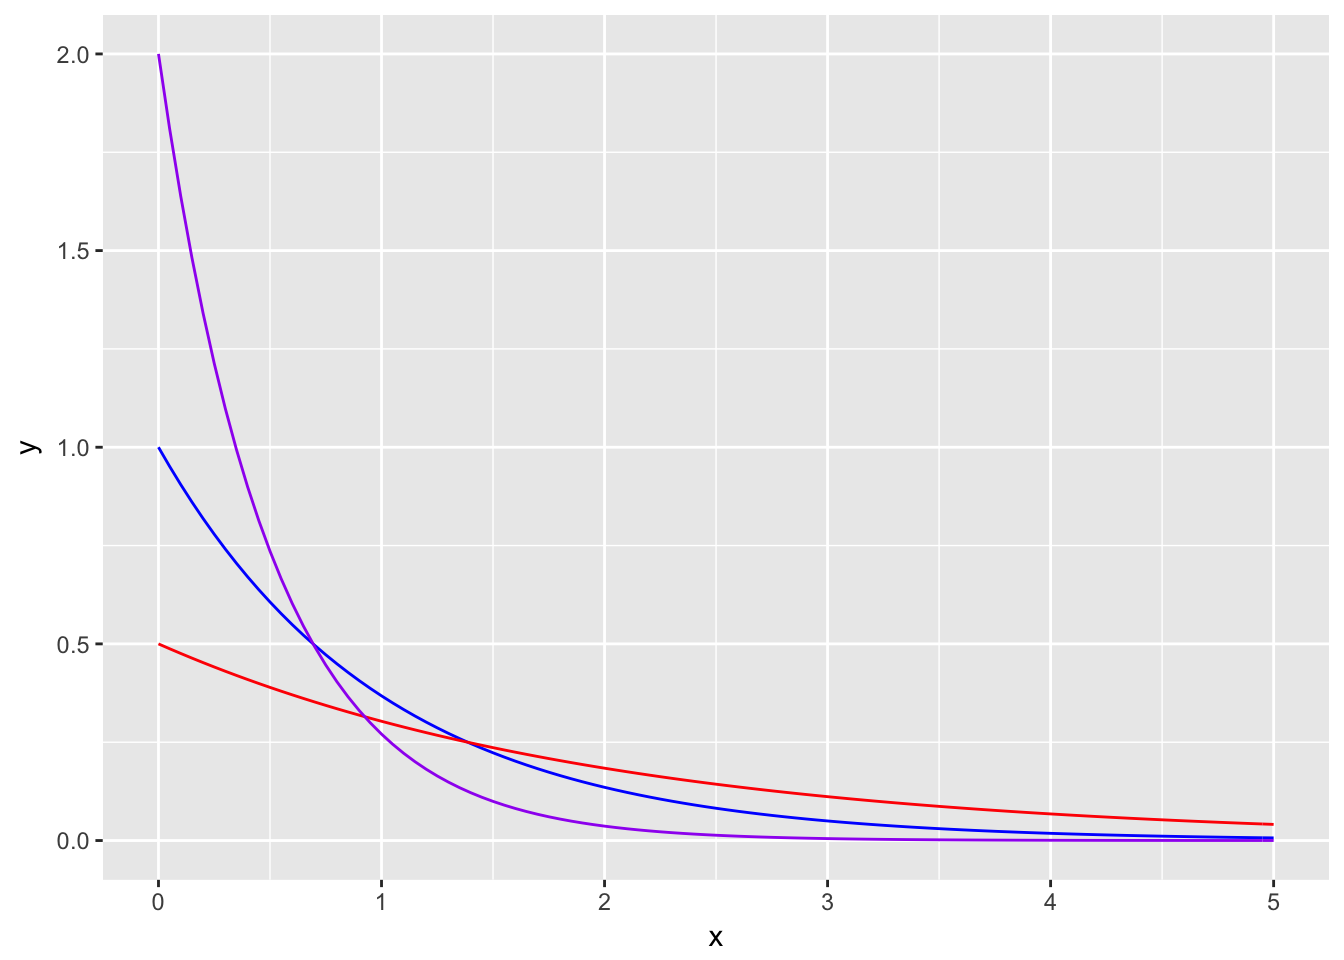
\includegraphics{book-of-prob_files/figure-latex/exp-1.pdf}

Example: Lifetime of a bulb is expected to be 10,000 hours, estimated
with exponential distribution. What is the probability that the bulb
will fail in the first 3,000 hours?

\[\lambda = 1/10^5\]

\[P(X < 3,000) = 1 - e^{-\lambda x} = 1 - e^{- 10^{-5}*3*10^3} = 0.0296\]

Example: Using the same properties of the question above, what is the
probability that the bulb will last more than 7,000 hours if it didn't
fail in the first 5,000 hours?

From memoryless property.

\[P(X > 7000 | X > 5000) = P(X > 5000 + 2000)/P(X>5000) = P(X > 2000) = e^{-\lambda x} = 0.9801987\]

\hypertarget{normal-distribution}{%
\section{Normal Distribution}\label{normal-distribution}}

It is the most popular continuous distribution with uniform distribution
and it has many applications. Also several discrete and continuous
distributions (i.e.~Binomial, t and chi-squared) converge to normal
distribution when data size increases. It is also called Gaussian
distribution. Many miscalculations or failed prediction happen because
people approximate empirical distributions to normal distribution. It
has two main parameters mean (location) \(\mu\) and standard deviation
(scale) \(\sigma\).

\[X \sim N(\mu,\sigma)\]

\begin{itemize}
\item
  Density:
  \(f(X) = \dfrac{1}{\sqrt{2\pi}\sigma}e^{-\dfrac{1}{2\sigma^2}(x-\mu)^2}\)
\item
  \(E[X] = \mu\)
\item
  \(V(X) = \sigma^2\)
\end{itemize}

If \(X \sim N(0,1)\), it is called standard normal distribution.

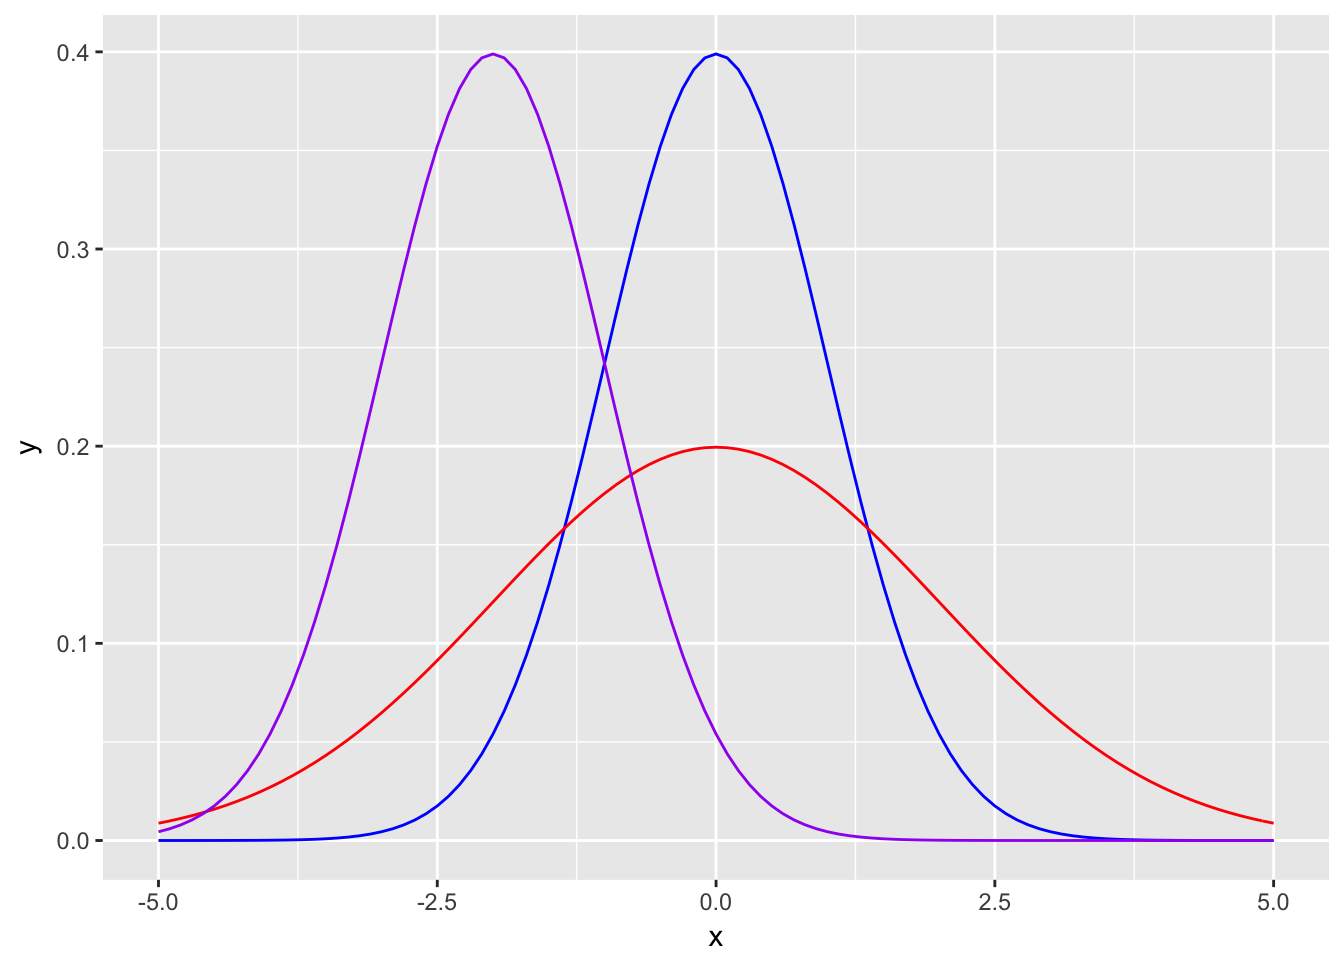
\includegraphics{book-of-prob_files/figure-latex/norm-1.pdf}

\hypertarget{standard-normal-distribution}{%
\subsection{Standard Normal
Distribution}\label{standard-normal-distribution}}

Standard Normal Distribution is a special case of normal distribution
with mean (\(\mu\)) 0 and standard deviation (\(\sigma\)) 1
\(X ~ N(0,1)\). Probability calculations in normal distribution is
usually done with converting the parameters to standard normal
parameters and finding the probabilities from the standard normal table
(or z-table). Conversion to standard normal is done as follows.
(\emph{You can find the z-table on course website.})

\[\dfrac{X-\mu}{\sigma}\]

Example: In a population height of the individuals are normally
distributed with mean 170cm and standard deviation 5cm. What is the
probability of a randomly selected person's height is 160cm or lower?

Solution:
\(P(X < 160; \mu = 170, \sigma = 5) = P(X < \dfrac{160 - 170}{5}) = \phi(-2) = 0.0228\).

\hypertarget{gamma-distribution}{%
\section{Gamma Distribution}\label{gamma-distribution}}

First, let's define the gamma function.

\[\Gamma(n) = \int_0^\infty x^{n-1}e^{-x}dx\]

By extensions there are some interesting properties.

\[\Gamma(n) = (n-1)\Gamma(n-1)\]

If n is a positive integer then \[\Gamma(n) = (n-1)!\].

You can use Gamma Distribution in reliability calculations with multiple
components.

\begin{itemize}
\item
  Density:
  \(f(X) = \dfrac{\lambda}{\Gamma(r)}(\lambda x)^{r-1} e^{-\lambda x}, x > 0\).
\item
  \(E[X] = r/\lambda\)
\item
  \(V(X) = r/\lambda^2\)
\end{itemize}

Exponential distribution is a special case of Gamma distribution with
\(r=1\).

\hypertarget{weibull-distribution}{%
\section{Weibull Distribution}\label{weibull-distribution}}

Some application of Weibull distribution are to estimate the time for
failure in multi component electrical or mechanical systems, and
modelling wind speed.

\begin{itemize}
\item
  Density:
  \(f(X) = \dfrac{\beta}{\delta}\left(\dfrac{x - \gamma}{\delta}\right)^{\beta-1} e^{-\left(\dfrac{x - \gamma}{\delta}\right)^\beta}\).
\item
  CDF: \(F(X) = 1 - e^{-\left(\dfrac{x - \gamma}{\delta}\right)^\beta}\)
\item
  \(E[X] = \gamma + \delta \Gamma(1 + 1/\beta)\)
\item
  \(V(X) = \delta^2\left[\Gamma\left(1+\dfrac{2}{\beta}\right) - \left[\Gamma\left(1 + \dfrac{1}{\beta}\right)\right]^2 \right]\)
\end{itemize}

\hypertarget{r-functions}{%
\section{R Functions}\label{r-functions}}

R has predefined functions for virtually all distributions. Just write
\texttt{?Distributions} to the console.

\hypertarget{mini-in-class-exercises}{%
\section{Mini In-Class Exercises}\label{mini-in-class-exercises}}

\emph{These exercises are at will attempt questions. They will not be
graded, you will not turn in any submission.}

\begin{enumerate}
\def\labelenumi{\arabic{enumi}.}
\item
  Waiters in Çengelköy Çınaraltı Cafe, goes on a tea serving tour every
  5 minutes. What is the probability that a newly arrived customer waits
  between 2 and 3 minutes?
\item
  The waiting time at Çengelköy Börekçisi queue is exponentially
  distributed with a mean of 10 minutes. What is the probability that a
  customer would wait less than 8 minutes?
\item
  Suppose Z is a standard normal distributed random variable
  (\(Z ~ N(0,1)\)).

  \begin{enumerate}
  \def\labelenumii{\alph{enumii}.}
  \tightlist
  \item
    \(P(-0.2 \le Z \le 0.4) = ?\)
  \item
    If \(P(Z < k) = 0.0987\) what is \(k\)?
  \item
    If \(P(|Z| < k) = 0.95\) what is \(k\)?
  \end{enumerate}
\end{enumerate}

\hypertarget{joint-distributions}{%
\chapter{Joint Distributions}\label{joint-distributions}}

So far, we learned about joint probabilities in Bayesian context such as
\(P(A|B) = P(A,B)/P(B)\). Now, we are going to expand this concept into
discrete and continuous distributions. Define \(P(X = x, Y=y) = f(x,y)\)
as the probability mass function (discrete) or probability density
function (continuous).

Same probability laws apply to joint distributions as well.

\begin{itemize}
\tightlist
\item
  \(f(x,y) \ge 0\) for all \((x,y)\).
\item
  \(\sum_x \sum_y f(x,y) = 1\) or \(\int_x \int_y f(x,y) dx dy = 1\)
\end{itemize}

\textbf{Example (Discrete)}: Suppose there are 10 balls in a box; 3
white, 4 black and 3 red. Two balls are randomly selected. Let's say
random variable X is the number of white balls picked and r.v. Y is the
number of black balls picked. (a) Find the joint probability function
and (b) find the probabilities.

\begin{enumerate}
\def\labelenumi{(\alph{enumi})}
\tightlist
\item
  Let's first enumerate the alternatives. \((x,y)\) pair can be either
  of \((0,0),(0,1),(0,2),(1,1),(2,0),(1,0)\). Total number of
  alternatives are \(\binom{10}{2}\). To calculate, number of ways of
  getting 1 white and 1 black ball is
  \(\binom{3}{1}\binom{4}{1}\binom{3}{0}\). So, the probability will be
  \(\dfrac{\binom{3}{1}\binom{4}{1}\binom{3}{0}}{\binom{10}{2}}\). We
  can generalize it to a function.
\end{enumerate}

\[f(x,y) = \dfrac{\binom{3}{x}\binom{4}{y}\binom{3}{2-x-y}}{\binom{10}{2}}\]

Let's also make it into an R function

\begin{verbatim}
## [1] 0.2666667
\end{verbatim}

\begin{enumerate}
\def\labelenumi{(\alph{enumi})}
\setcounter{enumi}{1}
\tightlist
\item
  Using the above formula we can calculate all the probabilities within
  the specified region \(x+y \le 2\).
\end{enumerate}

\begin{verbatim}
##      x_0  x_1  x_2
## y_0 0.07 0.20 0.07
## y_1 0.27 0.27 0.00
## y_2 0.13 0.00 0.00
\end{verbatim}

\textbf{Example (continuous)}: \emph{(This is from the textbook, Example
3.15)} A privately owned business operates both a drive-in facility and
a walk-in facility. On a randomly selected day, let X and Y,
respectively, be the proportions of time that the drive-in and the
walk-in facilities are in use and suppose that the joint density
function of these random variables is

\[
f(x,y) = \dfrac{2}{5}(2x + 3y), 0 \le x \le 1, 0 \le y \le 1
\]

and 0 for other values of x and y.

\begin{enumerate}
\def\labelenumi{(\alph{enumi})}
\item
  Verify \(\int_x \int_y f(x,y) dx dy = 1\)
\item
  Find \(P[(X,Y) \in A]\), where
  \(A = \{(x,y)|0 < x < 1/2, 1/4 < y < 1/2\}\)
\item
  (see the book for the full calculations)
\end{enumerate}

\[
\int_x \int_y f(x,y) dx dy = \int_0^1 \int_0^1 \dfrac{2}{5}(2x+3y) dx dy = 1
\]

\begin{enumerate}
\def\labelenumi{(\alph{enumi})}
\tightlist
\item
  (see the book for the full calculations)
\end{enumerate}

\[
\int_x \int_y f(x,y) dx dy = \int_{1/4}^{1/2} \int_0^{1/2} \dfrac{2}{5}(2x+3y) dx dy = 13/160
\]

Example (with special distributions)

\begin{enumerate}
\def\labelenumi{\arabic{enumi}.}
\item
  Patients arrive at the doctor's office according to Poisson
  distribution with \(\lambda = 2\)/hour.

  \begin{enumerate}
  \def\labelenumii{\alph{enumii})}
  \tightlist
  \item
    What is the probability of getting less than or equal to 2 patients
    within 2 hours?
  \item
    Suppose each arriving patient has 50\% chance to bring a person to
    accompany. There are 10 seats in the waiting room. At least many
    hours should pass that there is at least 50\% probability that the
    waiting room is filled with patients and their relatives?
  \end{enumerate}
\end{enumerate}

\textbf{Solution}

\begin{enumerate}
\def\labelenumi{\alph{enumi})}
\tightlist
\item
  \(P(X\le 2|\lambda t = 2)= \sum_{i=0}^2 \dfrac{e^{-\lambda t}(\lambda t)^i}{i!}\)
\end{enumerate}

\begin{verbatim}
## [1] 0.2381033
\end{verbatim}

\begin{enumerate}
\def\labelenumi{\alph{enumi})}
\setcounter{enumi}{1}
\item
  First let's define the problem. Define \(n_p\) as the number of
  patients and \(n_c\) is the number of company. We want
  \(n_p + n_c \ge 10\) with probability 50\% or higher for a given
  \(t^*\). Or to paraphrase, we want \(n_p + n_c \le 9\) w.p. 50\% or
  lower.

  What is \(n_c\) affected by? \(n_p\). It is actually a binomial
  distribution problem.
  \(P(n_c = i|n_p) = \binom{n_p}{i} (0.5)^i*(0.5)^{n_p-i}\). It is even
  better if we use cdf
  \(P(n_c \le k|n_p) = \sum_{i=0}^{k} \binom{n_p}{i} (0.5)^i*(0.5)^{n_p-i}\).

  We know the arrival of the patients is distributed with poisson. So,
  \(P(n_p = j|\lambda t^*) = \dfrac{e^{-\lambda t}(\lambda t)^j}{j!}\).
  So
  \(P(j + k \le N) = \sum_{a=0}^j P(n_p = a|\lambda t^*)*P(n_c \le N-a | n_p = a)\).
  Remember it is always \(n_c \le n_p\).
\end{enumerate}

\begin{verbatim}
## [1] 0.8631867
\end{verbatim}

\begin{verbatim}
## [1] 0.5810261
\end{verbatim}

\begin{verbatim}
## [1] 0.4905249
\end{verbatim}

\hypertarget{marginal-distributions}{%
\subsection{Marginal Distributions}\label{marginal-distributions}}

You can get the marginal distributions by just summing up or integrating
the other random variable such as \(P(Y=y) = \sum_x f(x,y)\) or
\(f(y) = \int_x f(x,y) dx\). Let's calculate the marginal distribution
of black balls (rv Y) in the above example.

\begin{verbatim}
##      x_0  x_1  x_2
## y_0 0.07 0.20 0.07
## y_1 0.27 0.27 0.00
## y_2 0.13 0.00 0.00
\end{verbatim}

\begin{verbatim}
##       y_0       y_1       y_2 
## 0.3333333 0.5333333 0.1333333
\end{verbatim}

Marginal distribution of y in the second example is calculated as
follows.

\[\int_x \dfrac{2}{5}(2x+3y) dx = \dfrac{2(1+3y)}{5}\]

\hypertarget{conditional-distribution-1}{%
\subsection{Conditional Distribution}\label{conditional-distribution-1}}

Similar to Bayes' Rule, it is possible to calculate conditional
probabilities of joint distributions. Let's denote g(x) as the marginal
distribution of x and h(y) as the marginal distribution of y. The
formula of conditional distribution of x given y is as follows.

\[f(x|y) = f(x,y)/h(y)\]

Note that conditional distribution function is useless if x and y are
independent. (\(f(x|y)=f(x)\))

\hypertarget{conditional-expectation}{%
\chapter{Conditional Expectation}\label{conditional-expectation}}

We learned about conditional distributions, but what about expectations?
(\(E[X|Y=y]\))

\[
E[X|Y=y] = \sum_x x P(X=x|Y=y)
E[X|Y=y] = \int_x x f(x|y) dx
E[E[X|Y]] = \sum_y E[X|Y=y]P(Y=y) = E[X]
\]

\textbf{Example:} A mouse is put into a labyrinth with 3 passages, at
the end of the labyrinth there is cheese. First passage leads to the
cheese in 3 mins. Second passage delays the mouse for 5 minutes and
returns the mouse to the starting point. Third is the same as the second
but the travel time is 10 minutes. It is equally likely that the mouse
chooses any of those passages. What is the expected amount of time that
the mouse will get to cheese?

Say \(T\) is time and \(Y\) is the passage chosen.

\[E[T] = E[E[T|Y]] = 1/3 E[T|Y=1] + 1/3 E[T|Y=3] + 1/3 E[T|Y=3]\]

\[E[T|Y=1] = 3\] \[E[T|Y=2] = 5 + E[T]\] \[E[T|Y=3] = 10 + E[T]\]

\[E[T] = 1/3 (3 + 5 + E[T] + 10 + E[T]) = 18\]

\hypertarget{further-topics}{%
\chapter{Further Topics}\label{further-topics}}

\emph{(not included)}

\hypertarget{moment-generating-function-mgf}{%
\section{Moment Generating Function
(MGF)}\label{moment-generating-function-mgf}}

If we define a function \(g(X)=X^r\) of r.v. X, the expected value
\(E[g(X)]\) is called the rth moment about the origin.

\[E[X^r] = \sum_x x^r f(x)\]

\[E[X^r] = \int_x x^r f(x) dx\]

The first moment gives us the expectation \(E[X^1]\). With the second
moment \(E[X^2]\) we can calculate the variance
\(V(X) = E[X^2] - E[X]^2\).

The moment generating functon \(M_X(t)\) is defined as follows.

\[M_X(t) = E[e^{tX}] = \sum_x e^{tx} f(x)\]

\[M_X(t) = E[e^{tX}] = \int_x e^{tx} f(x) dx\]

If the sum or interval above converges, then MGF exists. If MGF exists
then all moments can be calculated using the following derivative.

\[\dfrac{d^rM_X(t)}{dt^r} = E[X^r], at\ t=0\]

For instance, the MGF of binomial distribution is
\(M_X(t) = \sum_0^n e^{tx} \binom{n}{x}p^xq^{n-x}\).

\hypertarget{covariance}{%
\section{Covariance}\label{covariance}}

We know about the variance (\(V(X) = \sigma_x^2\) =
E{[}(X-E{[}X{]})\^{}2{]}). But what about the variance of two random
variables? Then we talk about the \textbf{covariance} of the joint
distribution (\(V(X,Y) = E[(X-E[X])(Y-E[Y])]\)) or
(\(E[XY] - E[X]E[Y]\)).

\hypertarget{correlation}{%
\section{Correlation}\label{correlation}}

Simply put, it is the magnitude of (linear) relationship between random
processes X and Y. Correlation coefficient can be found by using
covariance and variances of the marginal distributions.
(\(\dfrac{\sigma_{XY}}{\sigma_X\sigma_Y}\)).

Correlation is frequently used to indicate the similarity between two
processes. Though, there is a popular saying that `correlation does not
imply causation', meaning seemingly correlated processes might actually
be independent. Ask your instructor (or Google) about `spurious
correlations'.

\hypertarget{appendix-appendix}{%
\appendix}


\hypertarget{appendix-a}{%
\chapter{Appendix A}\label{appendix-a}}

Solving normal distribution problems is quite easy if you remember some
simple items.

\hypertarget{item-1-standard-normal-distribution-and-z-table}{%
\section{Item 1: Standard Normal Distribution and
z-table}\label{item-1-standard-normal-distribution-and-z-table}}

Standard normal distribution is special case of normal distribution with
mean (\(\mu\)) of 0 and standard deviation (\(\sigma\)) of 1. The
cumulative distribution function (CDF) values (\(P(X \le x)\)) of std
normal distribution are given in the z-table.

Note: CDF of the standard normal is also denoted with
\(\Phi(x) = P(X \le x)\). Note 2: For those of you who did not grasp the
concept of CDF; it is basically the probability that the outcome of the
event is less than the value specified. For instance \(\Phi(0)\)

\hypertarget{item-2-convert-and-normal-process-to-standard-normal.}{%
\section{Item 2: Convert and normal process to standard
normal.}\label{item-2-convert-and-normal-process-to-standard-normal.}}

Suppose you have a process (say, you pour cream on cakes) with mean 50
and standard deviation 5 and you want to know the probability of getting
less than 52. Follow this formula.

\[\Phi \left(\dfrac{X-\mu}{\sigma}\right)\]

So in our case, \(\Phi \left(\dfrac{52-50}{5}\right) = \Phi(0.4)\).

\hypertarget{item-3-how-to-read-z-table.}{%
\section{Item 3: How to read
z-table.}\label{item-3-how-to-read-z-table.}}

In the z-table sum of row and column names gives us the value (\(x\))
and their corresponding value gives us the probability \(\Phi(x)\). In
our example
\(\Phi(0.4) = \Phi(row + column) = \Phi(0.4 + 0.00) = 0.6554\)

\begin{figure}
\begin{center}
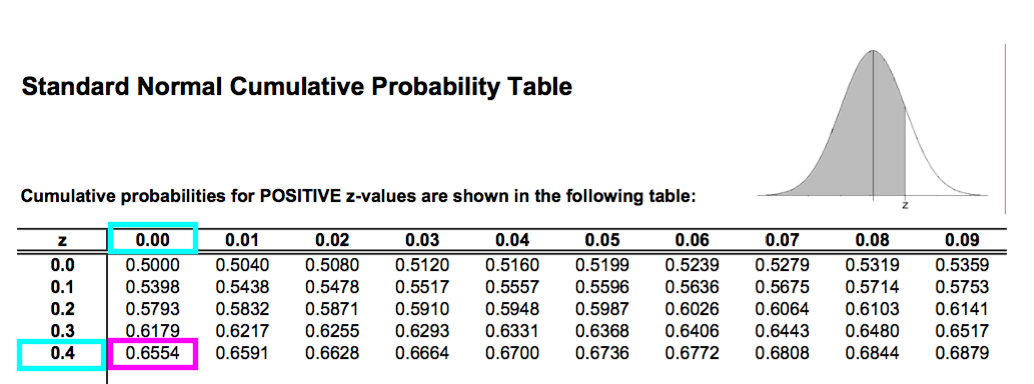
\includegraphics[width=0.95\columnwidth]{img/ss1}
\end{center}
\end{figure}

The notation for getting the (quantile) value is
\(\Phi^{-1}(0.6554) = 0.4\).

\hypertarget{item-4-symmetry}{%
\section{Item 4: Symmetry}\label{item-4-symmetry}}

The standard normal distribution is symmetric around 0. It gives us the
following useful property \(\Phi(-x) = 1 - \Phi(x)\). See
\(\Phi(-0.4) = 1 - 0.6554 = 0.3446\).

\begin{figure}
\begin{center}
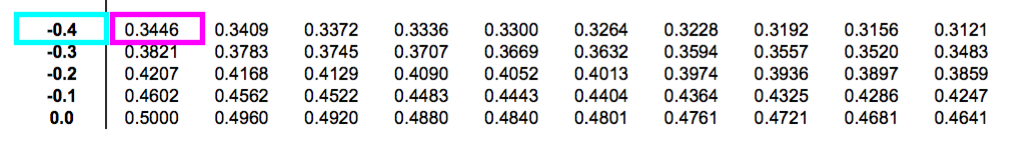
\includegraphics[width=0.95\columnwidth]{img/ss2}
\end{center}
\end{figure}

\hypertarget{item-5-understand-intervals.}{%
\section{Item 5: Understand
intervals.}\label{item-5-understand-intervals.}}

Due to the nature of normal distribution events mainly occur around the
mean. That's why central intervals are given with some probability
instead of from the bottom to the end. For instance suppose we would
like to know the probability around +-9.8 liters around the mean.

\[P(50 - 9.8 < X < 50 + 9.8) = P(40.2 < X < 59.8) = P(X < 59.8,X > 40,2) = P(X < 59.8) - P(X < 40.2)\]

Convert to standard normal.

\[P(X < (59.8 - 50)/5) - P(X < (40.2 - 50)/5) = \Phi(1.96) - \Phi(-1.96)\]

We know that \(\Phi(-x)= 1 - \Phi(x)\), so
\(\Phi(-1.96) = 1 - \Phi(1.96)\).

\[\Phi(1.96) - \Phi(-1.96) = \Phi(1.96) - (1 - \Phi(1.96)) = 2*\Phi(1.96) - 1\]

Check the z-table

\begin{figure}
\begin{center}
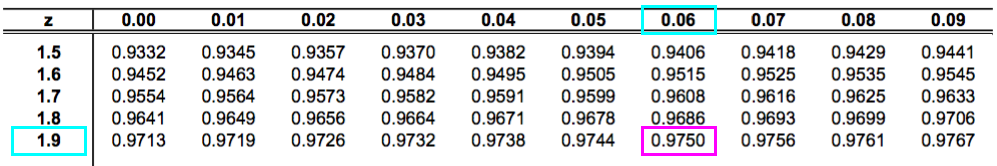
\includegraphics[width=0.95\columnwidth]{img/ss3}
\end{center}
\end{figure}

\(\Phi(1.96)\) is 0.975. So \(2*0.975 - 1 = 0.95\).

\hypertarget{item-6-moving-the-mean}{%
\section{Item 6: Moving the mean}\label{item-6-moving-the-mean}}

It is possible to desire an increased level of quality. For instance, if
we would like to have 90\% of the cakes have at least 50 grams of cream
instead of 50 grams just being the mean. So
\(P(X > 50) = 1 - P(X < 50) = 0.9\), then \(P(X < 50) = 0.1\). You have
the same standard deviation of 5 but you need a new mean.

\[\Phi \left(\dfrac{50 - \mu^*}{5}\right) = 0.1\]

We should invert the standard normal variate \(\Phi^{-1}(0.1)\). Let's
check the z-table for the values corresponding to 0.1.

\begin{figure}
\begin{center}
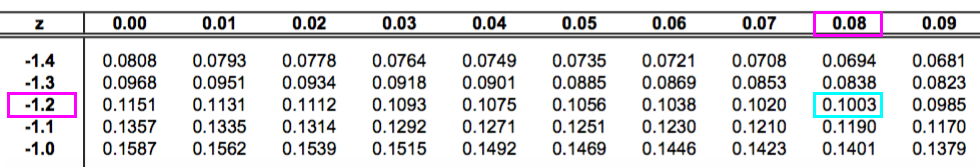
\includegraphics[width=0.95\columnwidth]{img/ss4}
\end{center}
\end{figure}

Well, closest value is 0.1003 so we go with it (usually linear
interpolation is done, but we'll skip that). The corresponding value is
-1.28.

\begin{align*}
\dfrac{50 - \mu^*}{5} &= -1.28 \\
50 - \mu^* &= -1.28*5 = -6.4 \\
\mu^* &= 50 + 6.4 = 56.4 \\
\end{align*}

So we should align ourself to pour 56.4 grams of cream per cake on
average in order to have 90\% of the cakes with 50 grams or more cream.

\hypertarget{conclusion}{%
\section{Conclusion}\label{conclusion}}

By the end of this tutorial you should know your way around the normal
distribution problems. It is not hard but you might need some practice
till you get adept on the topic.

\bibliography{book.bib,packages.bib}


\end{document}
